% Options for packages loaded elsewhere
\PassOptionsToPackage{unicode}{hyperref}
\PassOptionsToPackage{hyphens}{url}
%
\documentclass[
]{book}
\usepackage{amsmath,amssymb}
\usepackage{iftex}
\ifPDFTeX
  \usepackage[T1]{fontenc}
  \usepackage[utf8]{inputenc}
  \usepackage{textcomp} % provide euro and other symbols
\else % if luatex or xetex
  \usepackage{unicode-math} % this also loads fontspec
  \defaultfontfeatures{Scale=MatchLowercase}
  \defaultfontfeatures[\rmfamily]{Ligatures=TeX,Scale=1}
\fi
\usepackage{lmodern}
\ifPDFTeX\else
  % xetex/luatex font selection
\fi
% Use upquote if available, for straight quotes in verbatim environments
\IfFileExists{upquote.sty}{\usepackage{upquote}}{}
\IfFileExists{microtype.sty}{% use microtype if available
  \usepackage[]{microtype}
  \UseMicrotypeSet[protrusion]{basicmath} % disable protrusion for tt fonts
}{}
\makeatletter
\@ifundefined{KOMAClassName}{% if non-KOMA class
  \IfFileExists{parskip.sty}{%
    \usepackage{parskip}
  }{% else
    \setlength{\parindent}{0pt}
    \setlength{\parskip}{6pt plus 2pt minus 1pt}}
}{% if KOMA class
  \KOMAoptions{parskip=half}}
\makeatother
\usepackage{xcolor}
\usepackage{color}
\usepackage{fancyvrb}
\newcommand{\VerbBar}{|}
\newcommand{\VERB}{\Verb[commandchars=\\\{\}]}
\DefineVerbatimEnvironment{Highlighting}{Verbatim}{commandchars=\\\{\}}
% Add ',fontsize=\small' for more characters per line
\usepackage{framed}
\definecolor{shadecolor}{RGB}{248,248,248}
\newenvironment{Shaded}{\begin{snugshade}}{\end{snugshade}}
\newcommand{\AlertTok}[1]{\textcolor[rgb]{0.94,0.16,0.16}{#1}}
\newcommand{\AnnotationTok}[1]{\textcolor[rgb]{0.56,0.35,0.01}{\textbf{\textit{#1}}}}
\newcommand{\AttributeTok}[1]{\textcolor[rgb]{0.13,0.29,0.53}{#1}}
\newcommand{\BaseNTok}[1]{\textcolor[rgb]{0.00,0.00,0.81}{#1}}
\newcommand{\BuiltInTok}[1]{#1}
\newcommand{\CharTok}[1]{\textcolor[rgb]{0.31,0.60,0.02}{#1}}
\newcommand{\CommentTok}[1]{\textcolor[rgb]{0.56,0.35,0.01}{\textit{#1}}}
\newcommand{\CommentVarTok}[1]{\textcolor[rgb]{0.56,0.35,0.01}{\textbf{\textit{#1}}}}
\newcommand{\ConstantTok}[1]{\textcolor[rgb]{0.56,0.35,0.01}{#1}}
\newcommand{\ControlFlowTok}[1]{\textcolor[rgb]{0.13,0.29,0.53}{\textbf{#1}}}
\newcommand{\DataTypeTok}[1]{\textcolor[rgb]{0.13,0.29,0.53}{#1}}
\newcommand{\DecValTok}[1]{\textcolor[rgb]{0.00,0.00,0.81}{#1}}
\newcommand{\DocumentationTok}[1]{\textcolor[rgb]{0.56,0.35,0.01}{\textbf{\textit{#1}}}}
\newcommand{\ErrorTok}[1]{\textcolor[rgb]{0.64,0.00,0.00}{\textbf{#1}}}
\newcommand{\ExtensionTok}[1]{#1}
\newcommand{\FloatTok}[1]{\textcolor[rgb]{0.00,0.00,0.81}{#1}}
\newcommand{\FunctionTok}[1]{\textcolor[rgb]{0.13,0.29,0.53}{\textbf{#1}}}
\newcommand{\ImportTok}[1]{#1}
\newcommand{\InformationTok}[1]{\textcolor[rgb]{0.56,0.35,0.01}{\textbf{\textit{#1}}}}
\newcommand{\KeywordTok}[1]{\textcolor[rgb]{0.13,0.29,0.53}{\textbf{#1}}}
\newcommand{\NormalTok}[1]{#1}
\newcommand{\OperatorTok}[1]{\textcolor[rgb]{0.81,0.36,0.00}{\textbf{#1}}}
\newcommand{\OtherTok}[1]{\textcolor[rgb]{0.56,0.35,0.01}{#1}}
\newcommand{\PreprocessorTok}[1]{\textcolor[rgb]{0.56,0.35,0.01}{\textit{#1}}}
\newcommand{\RegionMarkerTok}[1]{#1}
\newcommand{\SpecialCharTok}[1]{\textcolor[rgb]{0.81,0.36,0.00}{\textbf{#1}}}
\newcommand{\SpecialStringTok}[1]{\textcolor[rgb]{0.31,0.60,0.02}{#1}}
\newcommand{\StringTok}[1]{\textcolor[rgb]{0.31,0.60,0.02}{#1}}
\newcommand{\VariableTok}[1]{\textcolor[rgb]{0.00,0.00,0.00}{#1}}
\newcommand{\VerbatimStringTok}[1]{\textcolor[rgb]{0.31,0.60,0.02}{#1}}
\newcommand{\WarningTok}[1]{\textcolor[rgb]{0.56,0.35,0.01}{\textbf{\textit{#1}}}}
\usepackage{longtable,booktabs,array}
\usepackage{calc} % for calculating minipage widths
% Correct order of tables after \paragraph or \subparagraph
\usepackage{etoolbox}
\makeatletter
\patchcmd\longtable{\par}{\if@noskipsec\mbox{}\fi\par}{}{}
\makeatother
% Allow footnotes in longtable head/foot
\IfFileExists{footnotehyper.sty}{\usepackage{footnotehyper}}{\usepackage{footnote}}
\makesavenoteenv{longtable}
\usepackage{graphicx}
\makeatletter
\def\maxwidth{\ifdim\Gin@nat@width>\linewidth\linewidth\else\Gin@nat@width\fi}
\def\maxheight{\ifdim\Gin@nat@height>\textheight\textheight\else\Gin@nat@height\fi}
\makeatother
% Scale images if necessary, so that they will not overflow the page
% margins by default, and it is still possible to overwrite the defaults
% using explicit options in \includegraphics[width, height, ...]{}
\setkeys{Gin}{width=\maxwidth,height=\maxheight,keepaspectratio}
% Set default figure placement to htbp
\makeatletter
\def\fps@figure{htbp}
\makeatother
\setlength{\emergencystretch}{3em} % prevent overfull lines
\providecommand{\tightlist}{%
  \setlength{\itemsep}{0pt}\setlength{\parskip}{0pt}}
\setcounter{secnumdepth}{5}
\usepackage{booktabs}
\usepackage{amsthm}
\makeatletter
\def\thm@space@setup{%
  \thm@preskip=8pt plus 2pt minus 4pt
  \thm@postskip=\thm@preskip
}
\makeatother
\ifLuaTeX
  \usepackage{selnolig}  % disable illegal ligatures
\fi
\usepackage[]{natbib}
\bibliographystyle{apalike}
\IfFileExists{bookmark.sty}{\usepackage{bookmark}}{\usepackage{hyperref}}
\IfFileExists{xurl.sty}{\usepackage{xurl}}{} % add URL line breaks if available
\urlstyle{same}
\hypersetup{
  pdftitle={MODELACIÓN DEL PRECIO PARA LA COMPRA Y VENTA DE ACEITE DE SOYA},
  pdfauthor={Nidia Munevar - Leonardo Palacios},
  hidelinks,
  pdfcreator={LaTeX via pandoc}}

\title{MODELACIÓN DEL PRECIO PARA LA COMPRA Y VENTA DE ACEITE DE SOYA}
\author{Nidia Munevar - Leonardo Palacios}
\date{2023-09-26}

\begin{document}
\maketitle

{
\setcounter{tocdepth}{1}
\tableofcontents
}
\hypertarget{resumen}{%
\chapter{Resumen}\label{resumen}}

El proyecto aplicado a realizar es la modelación del precio para la compra y venta de aceite de soya.

\hypertarget{introduccion}{%
\chapter{Introduccion}\label{introduccion}}

En el mercado de venta y compra de materias primas agrícolas intervienen diferentes actores, los precios son públicos y son afectados por diferentes variables tales como el precio del petróleo, la tasa de cambio, el clima entre otros elementos. La necesidad de los actores es mejorar sus decisiones y de esta forma su rentabilidad, los precios de las materias primas afectan directamente al mercado y a los precios de los bienes producidos a partir de estas, es decir estos valores terminan impactando al comprador final.

\hypertarget{justificacion}{%
\chapter{Justificacion}\label{justificacion}}

El proyecto está planteado ante una necesidad de los actores que requieren mejorar sus decisiones y de esta forma su rentabilidad. Los precios de las materias primas afectan directamente al mercado y a los precios de los bienes producidos a partir de estas materias, es decir estos valores terminan impactando al comprador final.

\hypertarget{serie-de-tiempo}{%
\chapter{Serie de Tiempo}\label{serie-de-tiempo}}

\begin{Shaded}
\begin{Highlighting}[]
\CommentTok{\# Cargar la biblioteca quantmod}
\FunctionTok{library}\NormalTok{(quantmod)}
\end{Highlighting}
\end{Shaded}

\begin{verbatim}
## Loading required package: xts
\end{verbatim}

\begin{verbatim}
## Loading required package: zoo
\end{verbatim}

\begin{verbatim}
## 
## Attaching package: 'zoo'
\end{verbatim}

\begin{verbatim}
## The following objects are masked from 'package:base':
## 
##     as.Date, as.Date.numeric
\end{verbatim}

\begin{verbatim}
## Loading required package: TTR
\end{verbatim}

\begin{verbatim}
## Registered S3 method overwritten by 'quantmod':
##   method            from
##   as.zoo.data.frame zoo
\end{verbatim}

\begin{Shaded}
\begin{Highlighting}[]
\CommentTok{\# Especificar el símbolo para futuros de soja}
\NormalTok{symbol }\OtherTok{\textless{}{-}} \StringTok{"ZS=F"}

\CommentTok{\# Descargar los datos históricos desde el 1 de enero de 2010 hasta hoy}
\FunctionTok{getSymbols}\NormalTok{(symbol, }\AttributeTok{from =} \StringTok{"2010{-}01{-}01"}\NormalTok{, }\AttributeTok{to =} \FunctionTok{Sys.Date}\NormalTok{(), }\AttributeTok{auto.assign =} \ConstantTok{TRUE}\NormalTok{)}
\end{Highlighting}
\end{Shaded}

\begin{verbatim}
## [1] "ZS=F"
\end{verbatim}

\begin{Shaded}
\begin{Highlighting}[]
\CommentTok{\# Crear un data frame con la serie de tiempo}
\NormalTok{soybean\_data }\OtherTok{\textless{}{-}} \FunctionTok{data.frame}\NormalTok{(}\AttributeTok{Date =} \FunctionTok{index}\NormalTok{(}\FunctionTok{get}\NormalTok{(symbol)), }
                           \AttributeTok{Open =} \FunctionTok{Op}\NormalTok{(}\FunctionTok{get}\NormalTok{(symbol)),}
                           \AttributeTok{High =} \FunctionTok{Hi}\NormalTok{(}\FunctionTok{get}\NormalTok{(symbol)),}
                           \AttributeTok{Low =} \FunctionTok{Lo}\NormalTok{(}\FunctionTok{get}\NormalTok{(symbol)),}
                           \AttributeTok{Close =} \FunctionTok{Cl}\NormalTok{(}\FunctionTok{get}\NormalTok{(symbol)),}
                           \AttributeTok{Volume =} \FunctionTok{Vo}\NormalTok{(}\FunctionTok{get}\NormalTok{(symbol))}
\NormalTok{                           )}

\CommentTok{\# Eliminar filas con valores NA}
\NormalTok{soybean\_data }\OtherTok{\textless{}{-}} \FunctionTok{na.omit}\NormalTok{(soybean\_data)}

\CommentTok{\# Muestra los primeros registros del data frame}
\FunctionTok{head}\NormalTok{(soybean\_data)}
\end{Highlighting}
\end{Shaded}

\begin{verbatim}
##                  Date ZS.F.Open ZS.F.High ZS.F.Low ZS.F.Close ZS.F.Volume
## 2010-01-04 2010-01-04   1043.00   1065.50  1041.25    1049.50       25947
## 2010-01-05 2010-01-05   1047.00   1056.00  1042.00    1052.25       21073
## 2010-01-06 2010-01-06   1050.00   1058.50  1042.75    1050.50       17567
## 2010-01-07 2010-01-07   1050.50   1052.00  1016.50    1017.75       11750
## 2010-01-08 2010-01-08   1018.25   1018.25  1005.00    1013.00       11750
## 2010-01-11 2010-01-11   1014.00   1022.00   997.50    1001.75       11750
\end{verbatim}

\begin{Shaded}
\begin{Highlighting}[]
\FunctionTok{class}\NormalTok{(soybean\_data)}
\end{Highlighting}
\end{Shaded}

\begin{verbatim}
## [1] "data.frame"
\end{verbatim}

\begin{Shaded}
\begin{Highlighting}[]
\CommentTok{\# Cargar la biblioteca xts}
\FunctionTok{library}\NormalTok{(xts)}

\CommentTok{\# Crear una serie de tiempo xts a partir del data frame soybean\_data}
\NormalTok{soybean\_xts }\OtherTok{\textless{}{-}} \FunctionTok{xts}\NormalTok{(soybean\_data[, }\SpecialCharTok{{-}}\DecValTok{1}\NormalTok{], }\AttributeTok{order.by =}\NormalTok{ soybean\_data}\SpecialCharTok{$}\NormalTok{Date)}

\CommentTok{\# Verificar la serie de tiempo}
\FunctionTok{head}\NormalTok{(soybean\_xts)}
\end{Highlighting}
\end{Shaded}

\begin{verbatim}
##            ZS.F.Open ZS.F.High ZS.F.Low ZS.F.Close ZS.F.Volume
## 2010-01-04   1043.00   1065.50  1041.25    1049.50       25947
## 2010-01-05   1047.00   1056.00  1042.00    1052.25       21073
## 2010-01-06   1050.00   1058.50  1042.75    1050.50       17567
## 2010-01-07   1050.50   1052.00  1016.50    1017.75       11750
## 2010-01-08   1018.25   1018.25  1005.00    1013.00       11750
## 2010-01-11   1014.00   1022.00   997.50    1001.75       11750
\end{verbatim}

\begin{Shaded}
\begin{Highlighting}[]
\FunctionTok{class}\NormalTok{(soybean\_xts)}
\end{Highlighting}
\end{Shaded}

\begin{verbatim}
## [1] "xts" "zoo"
\end{verbatim}

\hypertarget{analisis-exploratorio}{%
\chapter{Analisis Exploratorio}\label{analisis-exploratorio}}

\begin{Shaded}
\begin{Highlighting}[]
\CommentTok{\# Cargar la biblioteca quantmod}
\FunctionTok{library}\NormalTok{(quantmod)}

\CommentTok{\# Especificar el símbolo para futuros de soja}
\NormalTok{symbol }\OtherTok{\textless{}{-}} \StringTok{"ZS=F"}

\CommentTok{\# Descargar los datos históricos desde el 1 de enero de 2010 hasta hoy}
\FunctionTok{getSymbols}\NormalTok{(symbol, }\AttributeTok{from =} \StringTok{"2010{-}01{-}01"}\NormalTok{, }\AttributeTok{to =} \FunctionTok{Sys.Date}\NormalTok{(), }\AttributeTok{auto.assign =} \ConstantTok{TRUE}\NormalTok{)}
\end{Highlighting}
\end{Shaded}

\begin{verbatim}
## [1] "ZS=F"
\end{verbatim}

\begin{Shaded}
\begin{Highlighting}[]
\CommentTok{\# Crear un data frame con la serie de tiempo}
\NormalTok{soybean\_data }\OtherTok{\textless{}{-}} \FunctionTok{data.frame}\NormalTok{(}\AttributeTok{Date =} \FunctionTok{index}\NormalTok{(}\FunctionTok{get}\NormalTok{(symbol)), }
                           \AttributeTok{Open =} \FunctionTok{Op}\NormalTok{(}\FunctionTok{get}\NormalTok{(symbol)),}
                           \AttributeTok{High =} \FunctionTok{Hi}\NormalTok{(}\FunctionTok{get}\NormalTok{(symbol)),}
                           \AttributeTok{Low =} \FunctionTok{Lo}\NormalTok{(}\FunctionTok{get}\NormalTok{(symbol)),}
                           \AttributeTok{Close =} \FunctionTok{Cl}\NormalTok{(}\FunctionTok{get}\NormalTok{(symbol)),}
                           \AttributeTok{Volume =} \FunctionTok{Vo}\NormalTok{(}\FunctionTok{get}\NormalTok{(symbol))}
\NormalTok{)}

\CommentTok{\# Eliminar filas con valores NA}
\NormalTok{soybean\_data }\OtherTok{\textless{}{-}} \FunctionTok{na.omit}\NormalTok{(soybean\_data)}


\FunctionTok{head}\NormalTok{(soybean\_data)}
\end{Highlighting}
\end{Shaded}

\begin{verbatim}
##                  Date ZS.F.Open ZS.F.High ZS.F.Low ZS.F.Close ZS.F.Volume
## 2010-01-04 2010-01-04   1043.00   1065.50  1041.25    1049.50       25947
## 2010-01-05 2010-01-05   1047.00   1056.00  1042.00    1052.25       21073
## 2010-01-06 2010-01-06   1050.00   1058.50  1042.75    1050.50       17567
## 2010-01-07 2010-01-07   1050.50   1052.00  1016.50    1017.75       11750
## 2010-01-08 2010-01-08   1018.25   1018.25  1005.00    1013.00       11750
## 2010-01-11 2010-01-11   1014.00   1022.00   997.50    1001.75       11750
\end{verbatim}

\begin{Shaded}
\begin{Highlighting}[]
\CommentTok{\# Cargar la biblioteca xts}
\FunctionTok{library}\NormalTok{(xts)}

\CommentTok{\# Crear una serie de tiempo xts a partir del data frame soybean\_data}
\NormalTok{soybean\_xts }\OtherTok{\textless{}{-}} \FunctionTok{xts}\NormalTok{(soybean\_data[, }\SpecialCharTok{{-}}\DecValTok{1}\NormalTok{], }\AttributeTok{order.by =}\NormalTok{ soybean\_data}\SpecialCharTok{$}\NormalTok{Date)}

\CommentTok{\# Verificar la serie de tiempo}
\FunctionTok{head}\NormalTok{(soybean\_xts)}
\end{Highlighting}
\end{Shaded}

\begin{verbatim}
##            ZS.F.Open ZS.F.High ZS.F.Low ZS.F.Close ZS.F.Volume
## 2010-01-04   1043.00   1065.50  1041.25    1049.50       25947
## 2010-01-05   1047.00   1056.00  1042.00    1052.25       21073
## 2010-01-06   1050.00   1058.50  1042.75    1050.50       17567
## 2010-01-07   1050.50   1052.00  1016.50    1017.75       11750
## 2010-01-08   1018.25   1018.25  1005.00    1013.00       11750
## 2010-01-11   1014.00   1022.00   997.50    1001.75       11750
\end{verbatim}

\begin{Shaded}
\begin{Highlighting}[]
\FunctionTok{class}\NormalTok{(soybean\_xts)}
\end{Highlighting}
\end{Shaded}

\begin{verbatim}
## [1] "xts" "zoo"
\end{verbatim}

\begin{Shaded}
\begin{Highlighting}[]
\CommentTok{\# Acceder a la columna "ZS.F.Close" en soybean\_xts}
\NormalTok{close\_prices }\OtherTok{\textless{}{-}}\NormalTok{ soybean\_xts[, }\StringTok{"ZS.F.Close"}\NormalTok{]}

\CommentTok{\# Imprimir las primeras filas de la columna Close}
\FunctionTok{print}\NormalTok{(}\FunctionTok{head}\NormalTok{(close\_prices))}
\end{Highlighting}
\end{Shaded}

\begin{verbatim}
##            ZS.F.Close
## 2010-01-04    1049.50
## 2010-01-05    1052.25
## 2010-01-06    1050.50
## 2010-01-07    1017.75
## 2010-01-08    1013.00
## 2010-01-11    1001.75
\end{verbatim}

\begin{Shaded}
\begin{Highlighting}[]
\FunctionTok{head}\NormalTok{(soybean\_xts)}
\end{Highlighting}
\end{Shaded}

\begin{verbatim}
##            ZS.F.Open ZS.F.High ZS.F.Low ZS.F.Close ZS.F.Volume
## 2010-01-04   1043.00   1065.50  1041.25    1049.50       25947
## 2010-01-05   1047.00   1056.00  1042.00    1052.25       21073
## 2010-01-06   1050.00   1058.50  1042.75    1050.50       17567
## 2010-01-07   1050.50   1052.00  1016.50    1017.75       11750
## 2010-01-08   1018.25   1018.25  1005.00    1013.00       11750
## 2010-01-11   1014.00   1022.00   997.50    1001.75       11750
\end{verbatim}

\begin{Shaded}
\begin{Highlighting}[]
\CommentTok{\# Cargar la biblioteca ggplot2 para hacer gráficos}
\FunctionTok{library}\NormalTok{(ggplot2)}
\end{Highlighting}
\end{Shaded}

\begin{verbatim}
## Warning: package 'ggplot2' was built under R version 4.2.3
\end{verbatim}

\begin{Shaded}
\begin{Highlighting}[]
\CommentTok{\# Crear un gráfico de serie de tiempo}
\FunctionTok{ggplot}\NormalTok{(}\AttributeTok{data =} \ConstantTok{NULL}\NormalTok{, }\FunctionTok{aes}\NormalTok{(}\AttributeTok{x =} \FunctionTok{index}\NormalTok{(close\_prices), }\AttributeTok{y =}\NormalTok{ close\_prices)) }\SpecialCharTok{+}
  \FunctionTok{geom\_line}\NormalTok{(}\AttributeTok{color =} \StringTok{"blue"}\NormalTok{) }\SpecialCharTok{+}
  \FunctionTok{labs}\NormalTok{(}\AttributeTok{x =} \StringTok{"Fecha"}\NormalTok{, }\AttributeTok{y =} \StringTok{"Precio de Cierre"}\NormalTok{, }\AttributeTok{title =} \StringTok{"Serie de Tiempo de Futuros de Soja"}\NormalTok{) }\SpecialCharTok{+}
  \FunctionTok{theme\_minimal}\NormalTok{()}
\end{Highlighting}
\end{Shaded}

\begin{verbatim}
## Don't know how to automatically pick scale for object of type <xts/zoo>.
## Defaulting to continuous.
\end{verbatim}

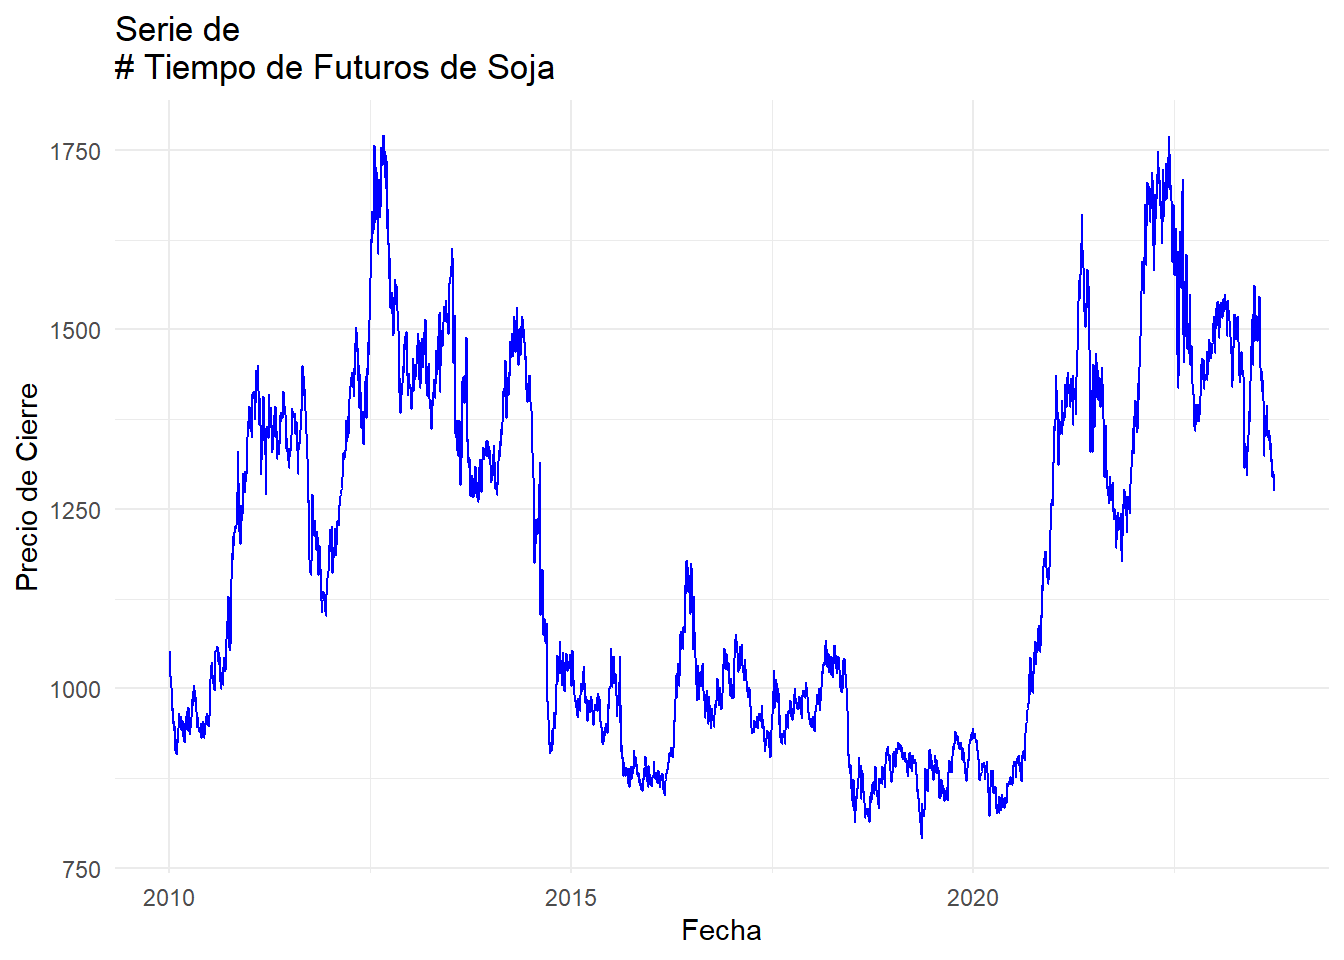
\includegraphics{bookdown-demo_files/figure-latex/unnamed-chunk-10-1.pdf}

\hypertarget{promedio-movil}{%
\chapter{Promedio Movil}\label{promedio-movil}}

Cuando aplicamos un promedio móvil a una serie de tiempo, cada punto de la serie transformada (promediada) es el promedio de un número determinado de puntos anteriores, actuales y futuros de la serie original. Este número de puntos que decides promediar se llama ``ventana'' del promedio móvil.

\begin{Shaded}
\begin{Highlighting}[]
\CommentTok{\# Cargar la biblioteca quantmod}
\FunctionTok{library}\NormalTok{(quantmod)}

\CommentTok{\# Especificar el símbolo para futuros de soja}
\NormalTok{symbol }\OtherTok{\textless{}{-}} \StringTok{"ZS=F"}

\CommentTok{\# Descargar los datos históricos desde el 1 de enero de 2010 hasta hoy}
\FunctionTok{getSymbols}\NormalTok{(symbol, }\AttributeTok{from =} \StringTok{"2010{-}01{-}01"}\NormalTok{, }\AttributeTok{to =} \FunctionTok{Sys.Date}\NormalTok{(), }\AttributeTok{auto.assign =} \ConstantTok{TRUE}\NormalTok{)}
\end{Highlighting}
\end{Shaded}

\begin{verbatim}
## Warning: ZS=F contains missing values. Some functions will not work if objects
## contain missing values in the middle of the series. Consider using na.omit(),
## na.approx(), na.fill(), etc to remove or replace them.
\end{verbatim}

\begin{verbatim}
## [1] "ZS=F"
\end{verbatim}

\begin{Shaded}
\begin{Highlighting}[]
\CommentTok{\# Crear un data frame con la serie de tiempo}
\NormalTok{soybean\_data }\OtherTok{\textless{}{-}} \FunctionTok{data.frame}\NormalTok{(}\AttributeTok{Date =} \FunctionTok{index}\NormalTok{(}\FunctionTok{get}\NormalTok{(symbol)), }
                           \AttributeTok{Open =} \FunctionTok{Op}\NormalTok{(}\FunctionTok{get}\NormalTok{(symbol)),}
                           \AttributeTok{High =} \FunctionTok{Hi}\NormalTok{(}\FunctionTok{get}\NormalTok{(symbol)),}
                           \AttributeTok{Low =} \FunctionTok{Lo}\NormalTok{(}\FunctionTok{get}\NormalTok{(symbol)),}
                           \AttributeTok{Close =} \FunctionTok{Cl}\NormalTok{(}\FunctionTok{get}\NormalTok{(symbol)),}
                           \AttributeTok{Volume =} \FunctionTok{Vo}\NormalTok{(}\FunctionTok{get}\NormalTok{(symbol))}
\NormalTok{                           )}

\CommentTok{\# Eliminar filas con valores NA}
\NormalTok{soybean\_data }\OtherTok{\textless{}{-}} \FunctionTok{na.omit}\NormalTok{(soybean\_data)}

\CommentTok{\# Muestra los primeros registros del data frame}
\CommentTok{\# head(soybean\_data)}
\end{Highlighting}
\end{Shaded}

\begin{Shaded}
\begin{Highlighting}[]
\CommentTok{\# Cargar la biblioteca xts}
\FunctionTok{library}\NormalTok{(xts)}

\CommentTok{\# Crear una serie de tiempo xts a partir del data frame soybean\_data}
\NormalTok{soybean\_xts }\OtherTok{\textless{}{-}} \FunctionTok{xts}\NormalTok{(soybean\_data[, }\SpecialCharTok{{-}}\DecValTok{1}\NormalTok{], }\AttributeTok{order.by =}\NormalTok{ soybean\_data}\SpecialCharTok{$}\NormalTok{Date)}

\CommentTok{\# Verificar la serie de tiempo}
\CommentTok{\# head(soybean\_xts)}
\end{Highlighting}
\end{Shaded}

\begin{Shaded}
\begin{Highlighting}[]
\FunctionTok{library}\NormalTok{(ggplot2)}
\FunctionTok{library}\NormalTok{(TTR)}
\FunctionTok{library}\NormalTok{(scales)}
\end{Highlighting}
\end{Shaded}

\begin{verbatim}
## Warning: package 'scales' was built under R version 4.2.3
\end{verbatim}

\begin{Shaded}
\begin{Highlighting}[]
\CommentTok{\# Convertir el objeto xts a data.frame}
\NormalTok{soybean\_df }\OtherTok{\textless{}{-}} \FunctionTok{as.data.frame}\NormalTok{(soybean\_xts)}
\NormalTok{soybean\_df}\SpecialCharTok{$}\NormalTok{Date }\OtherTok{\textless{}{-}} \FunctionTok{index}\NormalTok{(soybean\_xts)}

\CommentTok{\# Calcular SMA\_200 y SMA\_500}
\NormalTok{soybean\_df}\SpecialCharTok{$}\NormalTok{SMA\_200 }\OtherTok{\textless{}{-}} \FunctionTok{SMA}\NormalTok{(soybean\_df}\SpecialCharTok{$}\NormalTok{ZS.F.Close, }\AttributeTok{n =} \DecValTok{200}\NormalTok{)}
\NormalTok{soybean\_df}\SpecialCharTok{$}\NormalTok{SMA\_500 }\OtherTok{\textless{}{-}} \FunctionTok{SMA}\NormalTok{(soybean\_df}\SpecialCharTok{$}\NormalTok{ZS.F.Close, }\AttributeTok{n =} \DecValTok{500}\NormalTok{)}

\CommentTok{\# Usar ggplot2 para visualizar los datos}
\FunctionTok{ggplot}\NormalTok{(soybean\_df, }\FunctionTok{aes}\NormalTok{(}\AttributeTok{x =}\NormalTok{ Date)) }\SpecialCharTok{+}
  \FunctionTok{geom\_line}\NormalTok{(}\FunctionTok{aes}\NormalTok{(}\AttributeTok{y =}\NormalTok{ ZS.F.Close, }\AttributeTok{color =} \StringTok{\textquotesingle{}Precio de Cierre\textquotesingle{}}\NormalTok{), }\AttributeTok{alpha =} \FloatTok{0.75}\NormalTok{) }\SpecialCharTok{+}
  \FunctionTok{geom\_line}\NormalTok{(}\FunctionTok{aes}\NormalTok{(}\AttributeTok{y =}\NormalTok{ SMA\_200, }\AttributeTok{color =} \StringTok{\textquotesingle{}Promedio Móvil 200\textquotesingle{}}\NormalTok{), }\AttributeTok{size =} \DecValTok{1}\NormalTok{, }\AttributeTok{na.rm =} \ConstantTok{TRUE}\NormalTok{) }\SpecialCharTok{+}
  \FunctionTok{geom\_line}\NormalTok{(}\FunctionTok{aes}\NormalTok{(}\AttributeTok{y =}\NormalTok{ SMA\_500, }\AttributeTok{color =} \StringTok{\textquotesingle{}Promedio Móvil 500\textquotesingle{}}\NormalTok{), }\AttributeTok{size =} \DecValTok{1}\NormalTok{, }\AttributeTok{na.rm =} \ConstantTok{TRUE}\NormalTok{) }\SpecialCharTok{+}
  \FunctionTok{theme\_minimal}\NormalTok{(}\AttributeTok{base\_size =} \DecValTok{15}\NormalTok{) }\SpecialCharTok{+}
  \FunctionTok{labs}\NormalTok{(}\AttributeTok{title =} \StringTok{\textquotesingle{}Serie de Tiempo de Futuros de Soja\textquotesingle{}}\NormalTok{,}
       \AttributeTok{subtitle =} \StringTok{\textquotesingle{}Con Promedios Móviles de 200 y 500 Días\textquotesingle{}}\NormalTok{,}
       \AttributeTok{y =} \StringTok{\textquotesingle{}Precio de Cierre\textquotesingle{}}\NormalTok{) }\SpecialCharTok{+}
  \FunctionTok{theme}\NormalTok{(}\AttributeTok{axis.title.x =} \FunctionTok{element\_blank}\NormalTok{(),}
        \AttributeTok{axis.text.x =} \FunctionTok{element\_text}\NormalTok{(}\AttributeTok{size =} \DecValTok{10}\NormalTok{, }\AttributeTok{angle =} \DecValTok{90}\NormalTok{, }\AttributeTok{vjust =} \FloatTok{0.5}\NormalTok{),}
        \AttributeTok{plot.title =} \FunctionTok{element\_text}\NormalTok{(}\AttributeTok{hjust =} \FloatTok{0.5}\NormalTok{),}
        \AttributeTok{plot.subtitle =} \FunctionTok{element\_text}\NormalTok{(}\AttributeTok{hjust =} \FloatTok{0.5}\NormalTok{),}
        \AttributeTok{legend.position =} \StringTok{"bottom"}\NormalTok{) }\SpecialCharTok{+}
  \FunctionTok{scale\_x\_date}\NormalTok{(}\AttributeTok{date\_breaks =} \StringTok{"1 year"}\NormalTok{, }\AttributeTok{date\_labels =} \StringTok{"\%Y"}\NormalTok{) }\SpecialCharTok{+}
  \FunctionTok{scale\_y\_continuous}\NormalTok{(}\AttributeTok{labels =} \FunctionTok{dollar\_format}\NormalTok{()) }\SpecialCharTok{+}
  \FunctionTok{scale\_color\_manual}\NormalTok{(}\AttributeTok{values =} \FunctionTok{c}\NormalTok{(}\StringTok{\textquotesingle{}Precio de Cierre\textquotesingle{}} \OtherTok{=} \StringTok{\textquotesingle{}blue\textquotesingle{}}\NormalTok{, }\StringTok{\textquotesingle{}Promedio Móvil 200\textquotesingle{}} \OtherTok{=} \StringTok{\textquotesingle{}red\textquotesingle{}}\NormalTok{, }\StringTok{\textquotesingle{}Promedio Móvil 500\textquotesingle{}} \OtherTok{=} \StringTok{\textquotesingle{}green\textquotesingle{}}\NormalTok{),}
                     \AttributeTok{name =} \StringTok{""}\NormalTok{)}
\end{Highlighting}
\end{Shaded}

\begin{verbatim}
## Warning: Using `size` aesthetic for lines was deprecated in ggplot2 3.4.0.
## i Please use `linewidth` instead.
## This warning is displayed once every 8 hours.
## Call `lifecycle::last_lifecycle_warnings()` to see where this warning was
## generated.
\end{verbatim}

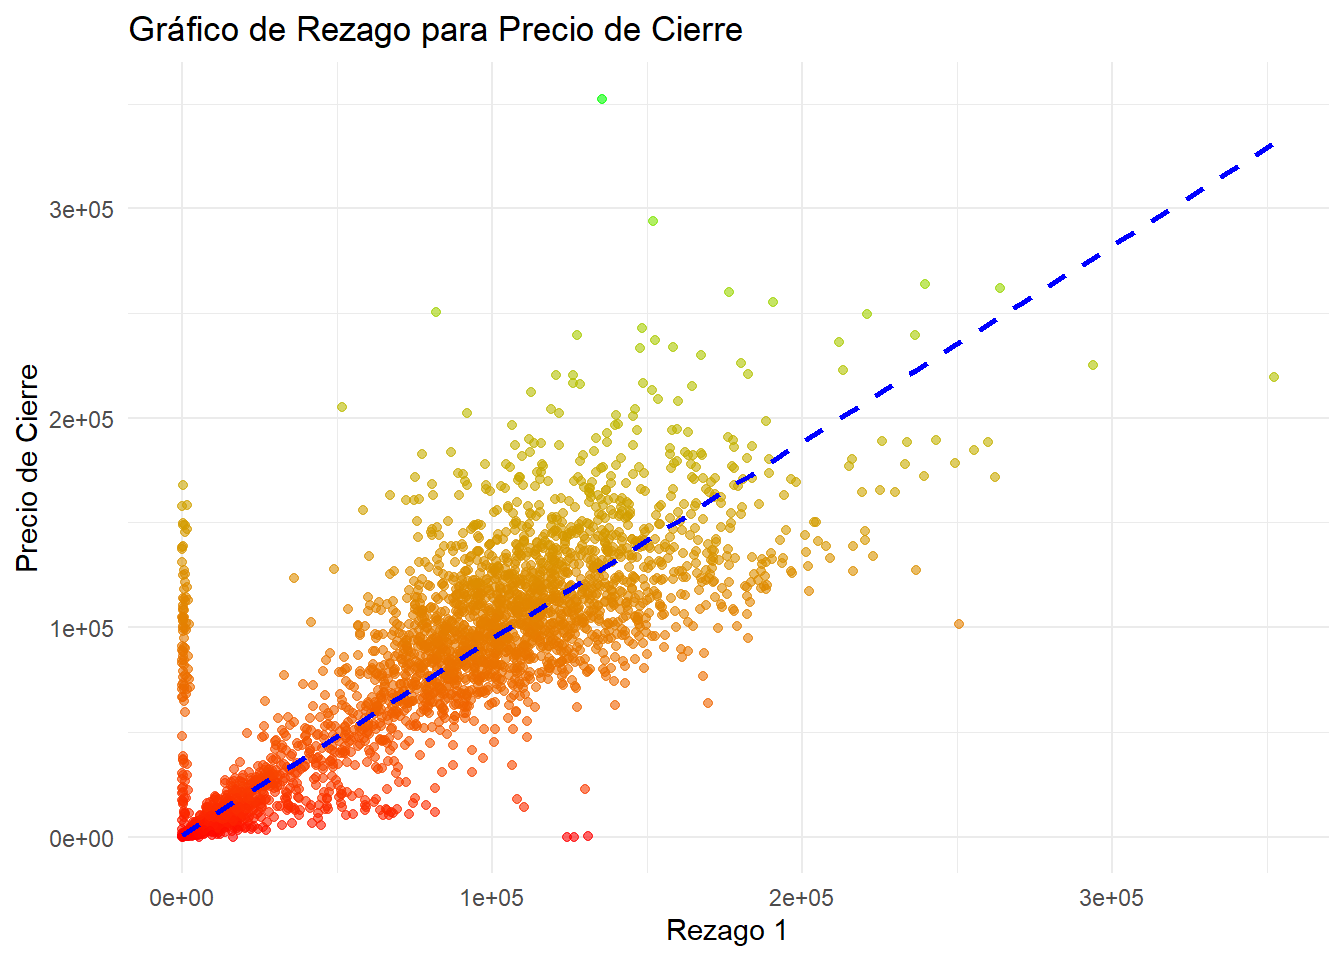
\includegraphics{bookdown-demo_files/figure-latex/unnamed-chunk-13-1.pdf}

Observaciones:

Entre los años 2013 y mediados del 2014 se puede ver cambios en la tendencia de la serie de tiempo de futuros de la soya, tamto para el promedio movil de 200 días, como para el de 500 días el cual es mas marcado.

Entre los años 2021 y mediados del 2023 se puede ver cambios en la tendencia de la serie de tiempo de futuros de la soya, tamto para el promedio movil de 200 días, como para el de 500 días el cual es mas marcado.Se podria llegar a validar por medio de un mayor estudio de este tiempo si la afectación fue causada por el desarrollo de la pandemia del covid-19 la cul inicio en marzo de 2020 e inicio a retrocer en Agosto de 2021 cuando se inicio el uso de las vacunas.

Al suavizar las fluctuaciones menores, a traves de los promedios móviles se logro resaltar las tendencias subyacentes en los datos.

\hypertarget{rezago}{%
\chapter{Rezago}\label{rezago}}

El concepto de rezago es fundamental para analizar y modelar series de tiempo porque permite entender cómo los valores pasados pueden influir en los valores presentes o futuros de la serie. Al analizar los rezagos, podemos identificar patrones, hacer predicciones más precisas y entender mejor la dinámica subyacente de los datos.

\begin{Shaded}
\begin{Highlighting}[]
\CommentTok{\# Sin cargar la librería dplyr para evitar conflictos}
\NormalTok{datos\_lag }\OtherTok{\textless{}{-}} \FunctionTok{data.frame}\NormalTok{(}
  \AttributeTok{Close =} \FunctionTok{as.numeric}\NormalTok{(}\FunctionTok{coredata}\NormalTok{(soybean\_xts)),}
  \AttributeTok{Lag =} \FunctionTok{as.numeric}\NormalTok{(}\FunctionTok{coredata}\NormalTok{(stats}\SpecialCharTok{::}\FunctionTok{lag}\NormalTok{(soybean\_xts))) }\CommentTok{\# Usar stats::lag para evitar conflictos}
\NormalTok{)}

\CommentTok{\# Comprobando que ambos vectores tengan la misma longitud}
\FunctionTok{stopifnot}\NormalTok{(}\FunctionTok{length}\NormalTok{(datos\_lag}\SpecialCharTok{$}\NormalTok{Close) }\SpecialCharTok{==} \FunctionTok{length}\NormalTok{(datos\_lag}\SpecialCharTok{$}\NormalTok{Lag))  }\CommentTok{\# Detiene la ejecución si no son TRUE}

\CommentTok{\# Crear el gráfico de rezago con ggplot2}
\FunctionTok{library}\NormalTok{(ggplot2)}
\FunctionTok{ggplot}\NormalTok{(datos\_lag, }\FunctionTok{aes}\NormalTok{(}\AttributeTok{x=}\NormalTok{Lag, }\AttributeTok{y=}\NormalTok{Close)) }\SpecialCharTok{+}
  \FunctionTok{geom\_point}\NormalTok{(}\FunctionTok{aes}\NormalTok{(}\AttributeTok{color =}\NormalTok{ Close), }\AttributeTok{alpha=}\FloatTok{0.6}\NormalTok{) }\SpecialCharTok{+}
  \FunctionTok{geom\_smooth}\NormalTok{(}\AttributeTok{method =} \StringTok{\textquotesingle{}lm\textquotesingle{}}\NormalTok{, }\AttributeTok{se =} \ConstantTok{FALSE}\NormalTok{, }\AttributeTok{color=}\StringTok{"blue"}\NormalTok{, }\AttributeTok{linetype=}\StringTok{"dashed"}\NormalTok{) }\SpecialCharTok{+}
  \FunctionTok{scale\_color\_gradient}\NormalTok{(}\AttributeTok{low=}\StringTok{"red"}\NormalTok{, }\AttributeTok{high=}\StringTok{"green"}\NormalTok{) }\SpecialCharTok{+}
  \FunctionTok{theme\_minimal}\NormalTok{() }\SpecialCharTok{+}
  \FunctionTok{labs}\NormalTok{(}\AttributeTok{title=}\StringTok{"Gráfico de Rezago para Precio de Cierre"}\NormalTok{, }\AttributeTok{x=}\StringTok{"Rezago 1"}\NormalTok{, }\AttributeTok{y=}\StringTok{"Precio de Cierre"}\NormalTok{) }\SpecialCharTok{+}
  \FunctionTok{theme}\NormalTok{(}\AttributeTok{legend.position=}\StringTok{"none"}\NormalTok{)}
\end{Highlighting}
\end{Shaded}

\begin{verbatim}
## `geom_smooth()` using formula = 'y ~ x'
\end{verbatim}

\begin{verbatim}
## Warning: Removed 5 rows containing non-finite values (`stat_smooth()`).
\end{verbatim}

\begin{verbatim}
## Warning: Removed 5 rows containing missing values (`geom_point()`).
\end{verbatim}

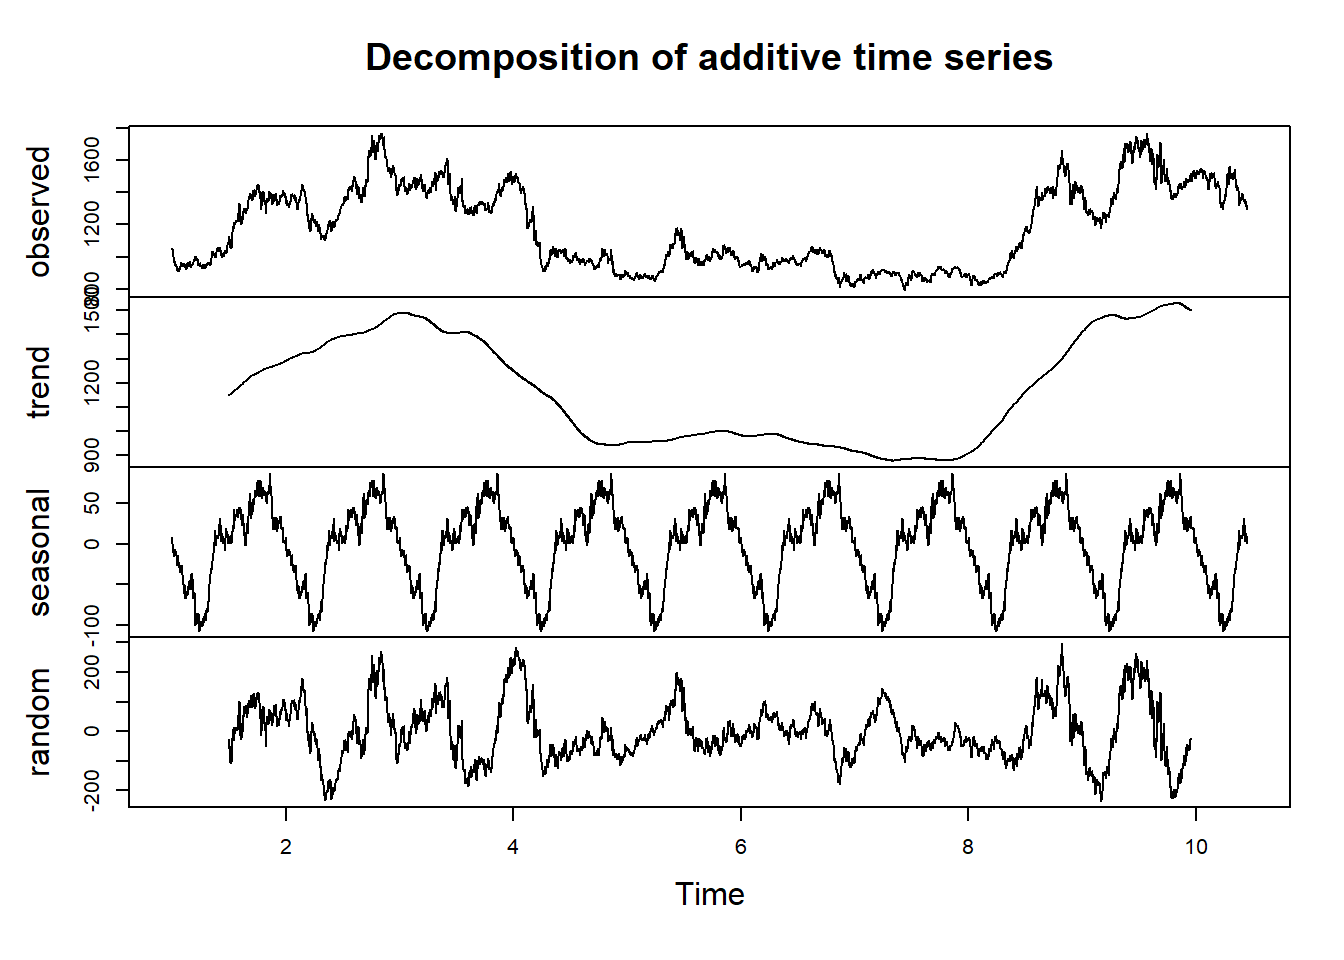
\includegraphics{bookdown-demo_files/figure-latex/unnamed-chunk-14-1.pdf}

Se ve un patrón claro o una agrupación de puntos en el gráfico de rezago 1, por lo tanto es probable que exista una autocorrelación significativa. Se puede considerar modelos de series de tiempo como ARIMA que toman en cuenta la autocorrelación para hacer predicciones más precisas de ser necesario.

\hypertarget{descomposicion}{%
\chapter{Descomposicion}\label{descomposicion}}

Se refiere a los patrones o tendencias que se repiten a intervalos regulares, como cada día, mes, trimestre o año, dependiendo de la frecuencia de los datos. En otras palabras, es como un ciclo que se repite en el tiempo.

DESCOMPOSICION

Con la funcion decompose podemos hallar la:

Observed: Serie de tiempo original.

Tendencia (trend): Muestra la dirección general en la que se mueven los datos a largo plazo, sin tener en cuenta las fluctuaciones estacionales o irregulares.

Estacionalidad (seasonal): Representa las fluctuaciones que ocurren en intervalos regulares, como los cambios diarios, mensuales o anuales, debido a la estacionalidad.

Error o Residuo (random): Es la parte de la serie de tiempo que no se puede atribuir ni a la tendencia ni a la estacionalidad. Captura la variabilidad en los datos que no se puede explicar por los otros dos componentes.

\begin{Shaded}
\begin{Highlighting}[]
\CommentTok{\# Convertir a objeto ts, aquí supondré que tienes datos diarios.}
\NormalTok{frecuencia }\OtherTok{\textless{}{-}} \DecValTok{365}  \CommentTok{\# (12 para mensual, 4 para trimestral, etc.)}
\NormalTok{soybean\_ts }\OtherTok{\textless{}{-}} \FunctionTok{ts}\NormalTok{(soybean\_xts[, }\StringTok{"ZS.F.Close"}\NormalTok{], }\AttributeTok{frequency =}\NormalTok{ frecuencia)}

\CommentTok{\# Utilizar decompose}
\NormalTok{soybean\_decomposed }\OtherTok{\textless{}{-}} \FunctionTok{decompose}\NormalTok{(soybean\_ts)}
\FunctionTok{plot}\NormalTok{(soybean\_decomposed)}
\end{Highlighting}
\end{Shaded}

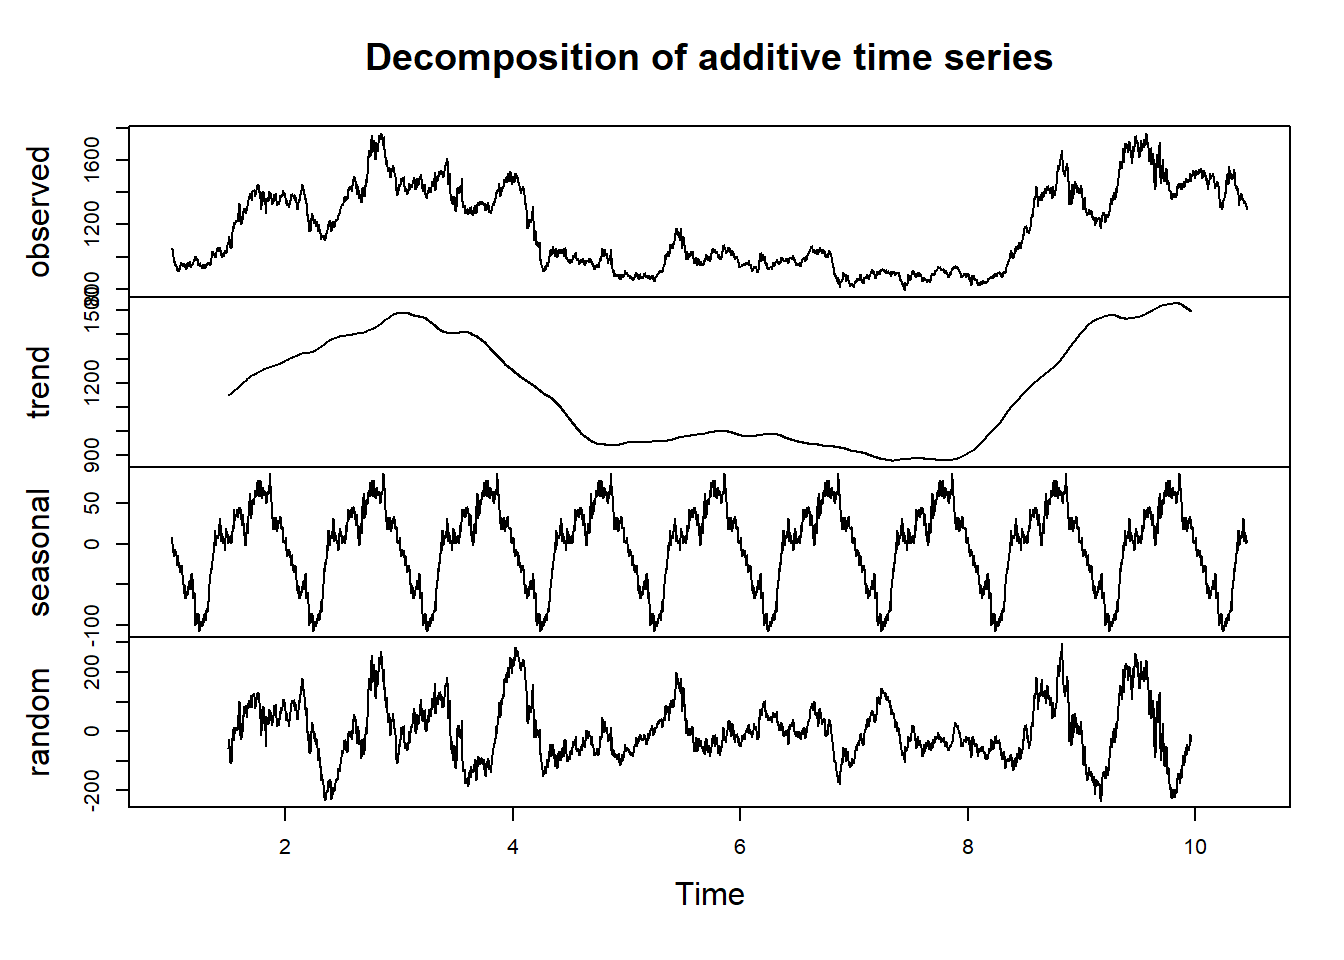
\includegraphics{bookdown-demo_files/figure-latex/unnamed-chunk-15-1.pdf}
Al validar el componenete estacional de la serie por separado, como se ve en la siguiente imagen:

\begin{Shaded}
\begin{Highlighting}[]
\CommentTok{\# Extraer el componente estacional y convertir el tiempo en fecha}
\NormalTok{seasonal\_df }\OtherTok{\textless{}{-}} \FunctionTok{data.frame}\NormalTok{(}
  \AttributeTok{Date =} \FunctionTok{as.Date}\NormalTok{(}\FunctionTok{index}\NormalTok{(soybean\_xts)),}
  \AttributeTok{Seasonal =} \FunctionTok{as.numeric}\NormalTok{(soybean\_decomposed}\SpecialCharTok{$}\NormalTok{seasonal)}
\NormalTok{)}

\CommentTok{\# Eliminar las filas con NA en el componente estacional (pueden aparecer dependiendo del método de descomposición)}
\NormalTok{seasonal\_df }\OtherTok{\textless{}{-}}\NormalTok{ seasonal\_df[}\SpecialCharTok{!}\FunctionTok{is.na}\NormalTok{(seasonal\_df}\SpecialCharTok{$}\NormalTok{Seasonal), ]}
\end{Highlighting}
\end{Shaded}

\begin{Shaded}
\begin{Highlighting}[]
\FunctionTok{library}\NormalTok{(ggplot2)}

\FunctionTok{ggplot}\NormalTok{(seasonal\_df, }\FunctionTok{aes}\NormalTok{(}\AttributeTok{x=}\NormalTok{Date, }\AttributeTok{y=}\NormalTok{Seasonal)) }\SpecialCharTok{+}
  \FunctionTok{geom\_line}\NormalTok{(}\AttributeTok{color=}\StringTok{"blue"}\NormalTok{) }\SpecialCharTok{+}
  \FunctionTok{theme\_minimal}\NormalTok{() }\SpecialCharTok{+}
  \FunctionTok{labs}\NormalTok{(}\AttributeTok{title=}\StringTok{"Componente Estacional de la Serie Temporal"}\NormalTok{, }\AttributeTok{x=}\StringTok{"Fecha"}\NormalTok{, }\AttributeTok{y=}\StringTok{"Estacionalidad"}\NormalTok{) }\SpecialCharTok{+}
  \FunctionTok{theme}\NormalTok{(}\AttributeTok{legend.position=}\StringTok{"none"}\NormalTok{)}
\end{Highlighting}
\end{Shaded}

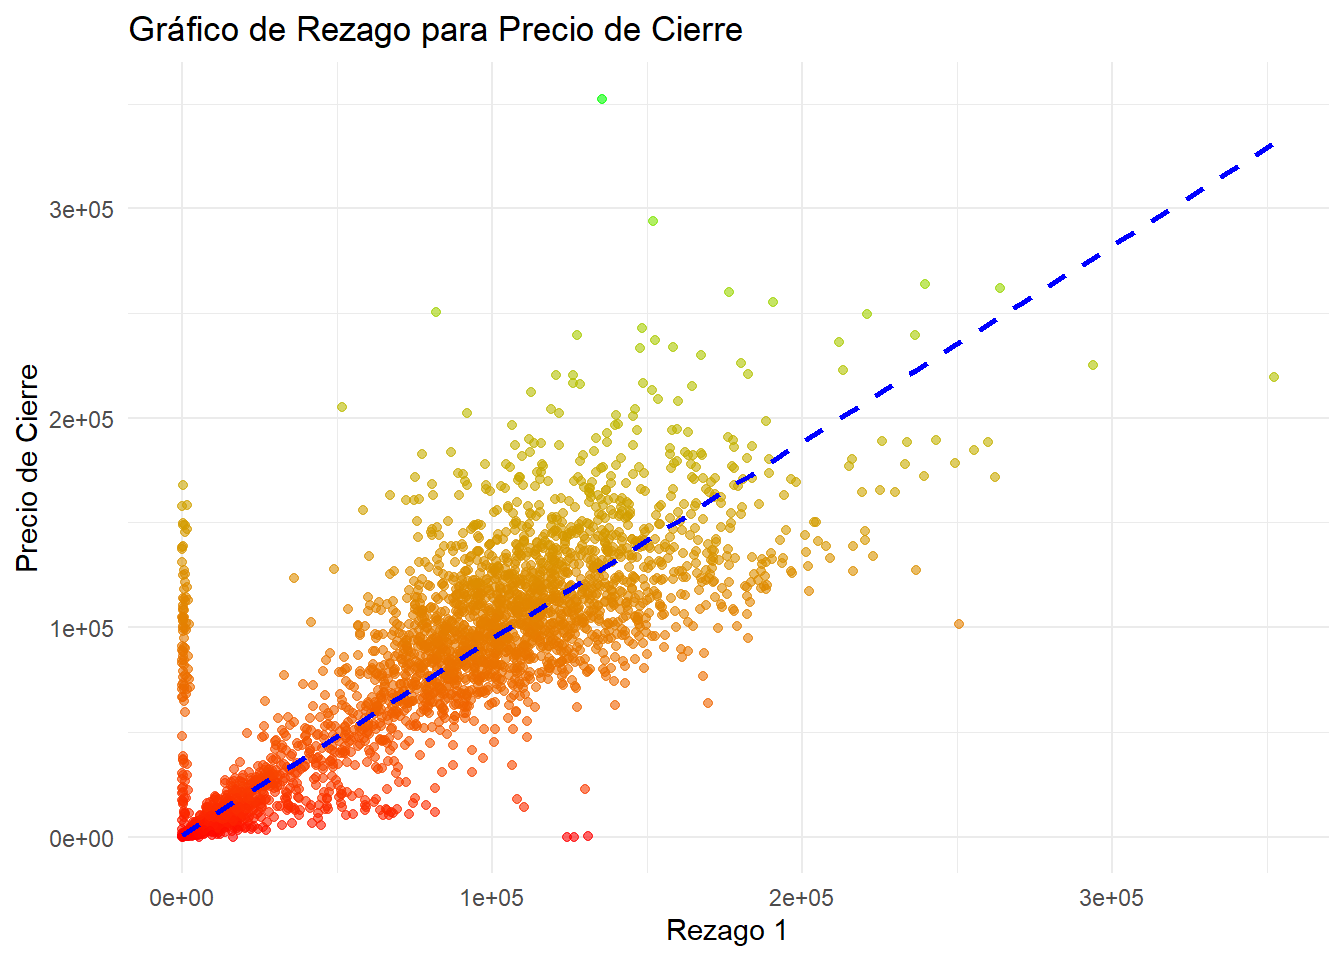
\includegraphics{bookdown-demo_files/figure-latex/unnamed-chunk-17-1.pdf}
Podemos deducir que la serie de tiempo de los precios del aceite de soya:

\begin{enumerate}
\def\labelenumi{\arabic{enumi}.}
\item
  Muestra patrones claros y consistentes, esto sugiere que la serie temporal tiene ciclos regulares que se repiten a intervalos fijos.
\item
  Se pueden identificar en qué momentos del ciclo tienden a ocurrir los valores altos y bajos de la serie.
\end{enumerate}

\hypertarget{estacionariedad}{%
\chapter{Estacionariedad}\label{estacionariedad}}

La prueba de Dickey-Fuller, específicamente el test ADF (Augmented Dickey-Fuller), es una prueba estadística utilizada para determinar si una serie temporal tiene una raíz unitaria, es decir, si es no estacionaria y presenta alguna forma de estructura temporal como una tendencia o una estacionalidad.

Vamos a comprobar mediante esta prueba si es o no estacionaria la serie de tiempo del precio del aceite de soya.

\begin{Shaded}
\begin{Highlighting}[]
\CommentTok{\# Cargar el paquete necesario}
\FunctionTok{library}\NormalTok{(tseries)}
\end{Highlighting}
\end{Shaded}

\begin{verbatim}
## Warning: package 'tseries' was built under R version 4.2.3
\end{verbatim}

\begin{Shaded}
\begin{Highlighting}[]
\CommentTok{\# Supón que tienes una serie temporal llamada \textquotesingle{}mi\_serie\textquotesingle{}}
\CommentTok{\# Realizar la prueba de Dickey{-}Fuller Aumentada}
\NormalTok{resultado\_adf }\OtherTok{\textless{}{-}} \FunctionTok{adf.test}\NormalTok{(soybean\_ts)}

\CommentTok{\# Imprimir el resultado}
\FunctionTok{print}\NormalTok{(resultado\_adf)}
\end{Highlighting}
\end{Shaded}

\begin{verbatim}
## 
##  Augmented Dickey-Fuller Test
## 
## data:  soybean_ts
## Dickey-Fuller = -2.0289, Lag order = 15, p-value = 0.5661
## alternative hypothesis: stationary
\end{verbatim}

Cuando hacemos una prueba como esta, estamos tratando de averiguar si la serie de tiempo es ``estacionaria'' o no. Una serie estacionaria es aquella cuyas propiedades, como la media y la varianza, no cambian con el tiempo.

En esta prueba, tenemos algo llamado valor p, que es como un termómetro que nos dice qué tan seguros estamos de si la serie de tiempo es estacionaria o no. Un valor p pequeño (menor que 0.05) nos dice: ``La serie es estacionaria''. Un valor p grande (mayor que 0.05) nos dice: ``La serie no es estacionaria''.

En este caso, el valor p es 0.5657, que es bastante grande, así que, la serie de tiempo no es estacionaria.

\hypertarget{diferenciacion}{%
\chapter{Diferenciacion}\label{diferenciacion}}

Diferenciar una serie temporal es un proceso utilizado para hacer que una serie no estacionaria se vuelva estacionaria. La idea es transformar la serie de datos para estabilizar la media de la serie temporal, eliminando tendencias y efectos estacionales. En otras palabras, se busca que las propiedades de la serie (como la media y la varianza) no cambien con el tiempo.

\begin{Shaded}
\begin{Highlighting}[]
\CommentTok{\# Inicializa un contador para las diferenciaciones}
\NormalTok{diferencias }\OtherTok{\textless{}{-}} \DecValTok{0}

\CommentTok{\# Realiza el test ADF y verifica la estacionariedad}
\ControlFlowTok{while}\NormalTok{(}\ConstantTok{TRUE}\NormalTok{) \{}
\NormalTok{  p\_value }\OtherTok{\textless{}{-}} \FunctionTok{adf.test}\NormalTok{(soybean\_ts)}\SpecialCharTok{$}\NormalTok{p.value}
  \FunctionTok{cat}\NormalTok{(}\StringTok{"Número de diferencias:"}\NormalTok{, diferencias, }\StringTok{"{-} Valor p:"}\NormalTok{, p\_value, }\StringTok{"}\SpecialCharTok{\textbackslash{}n}\StringTok{"}\NormalTok{)}
  
  \CommentTok{\# Si el valor p es menor que 0.05, la serie es estacionaria, y puedes salir del bucle.}
  \ControlFlowTok{if}\NormalTok{(p\_value }\SpecialCharTok{\textless{}} \FloatTok{0.05}\NormalTok{) \{}
    \FunctionTok{cat}\NormalTok{(}\StringTok{"La serie se volvió estacionaria después de"}\NormalTok{, diferencias, }\StringTok{"diferenciaciones.}\SpecialCharTok{\textbackslash{}n}\StringTok{"}\NormalTok{)}
    \ControlFlowTok{break}
\NormalTok{  \}}
  
  \CommentTok{\# Si has llegado al final de la serie, sal del bucle}
  \ControlFlowTok{if}\NormalTok{(}\FunctionTok{length}\NormalTok{(soybean\_ts) }\SpecialCharTok{\textless{}=} \DecValTok{1}\NormalTok{) \{}
    \FunctionTok{cat}\NormalTok{(}\StringTok{"La serie no se volvió estacionaria después de diferenciar.}\SpecialCharTok{\textbackslash{}n}\StringTok{"}\NormalTok{)}
    \ControlFlowTok{break}
\NormalTok{  \}}
  
  \CommentTok{\# Si no es estacionaria, diferenciar la serie una vez más y continuar el bucle.}
\NormalTok{  soybean\_ts }\OtherTok{\textless{}{-}} \FunctionTok{diff}\NormalTok{(soybean\_ts)}
\NormalTok{  diferencias }\OtherTok{\textless{}{-}}\NormalTok{ diferencias }\SpecialCharTok{+} \DecValTok{1}
\NormalTok{\}}
\end{Highlighting}
\end{Shaded}

\begin{verbatim}
## Número de diferencias: 0 - Valor p: 0.5660899
\end{verbatim}

\begin{verbatim}
## Warning in adf.test(soybean_ts): p-value smaller than printed p-value
\end{verbatim}

\begin{verbatim}
## Número de diferencias: 1 - Valor p: 0.01 
## La serie se volvió estacionaria después de 1 diferenciaciones.
\end{verbatim}

Conclusión:

Antes de realizar cualquier diferenciación (d = 0), el valor p de la prueba de Dickey-Fuller Aumentada es 0.5657422, lo que es mayor que 0.05. Por lo tanto, no puedes rechazar la hipótesis nula de que existe una raíz unitaria, y se concluye que la serie original no es estacionaria.

Después de diferenciar la serie una vez (d = 1), el valor p de la prueba de Dickey-Fuller Aumentada es 0.01, lo cual es menor que 0.05.

La serie de tiempo original no es estacionaria, pero después de realizar una diferenciación, la serie resultante sí es estacionaria.

Fue necesario transformarla o diferenciarla para eliminar la tendencia y estabilizar la varianza, antes de aplicar modelos de series temporales como ARIMA.

\hypertarget{holter-winter}{%
\chapter{Holter-Winter}\label{holter-winter}}

La metodología Holt-Winters, también conocida como triple suavizado exponencial, es útil para series de tiempo con componentes de tendencia y estacionalidad.

\begin{Shaded}
\begin{Highlighting}[]
\FunctionTok{library}\NormalTok{(forecast)  }\CommentTok{\# Necesario para pronosticar con el modelo Holt{-}Winters}
\end{Highlighting}
\end{Shaded}

\begin{verbatim}
## Warning: package 'forecast' was built under R version 4.2.3
\end{verbatim}

\begin{Shaded}
\begin{Highlighting}[]
\CommentTok{\# Ajustar el modelo Holt{-}Winters}
\NormalTok{hw\_model }\OtherTok{\textless{}{-}} \FunctionTok{HoltWinters}\NormalTok{(soybean\_ts)}
\CommentTok{\# Visualizar componentes del modelo}
\FunctionTok{plot}\NormalTok{(hw\_model)}
\end{Highlighting}
\end{Shaded}

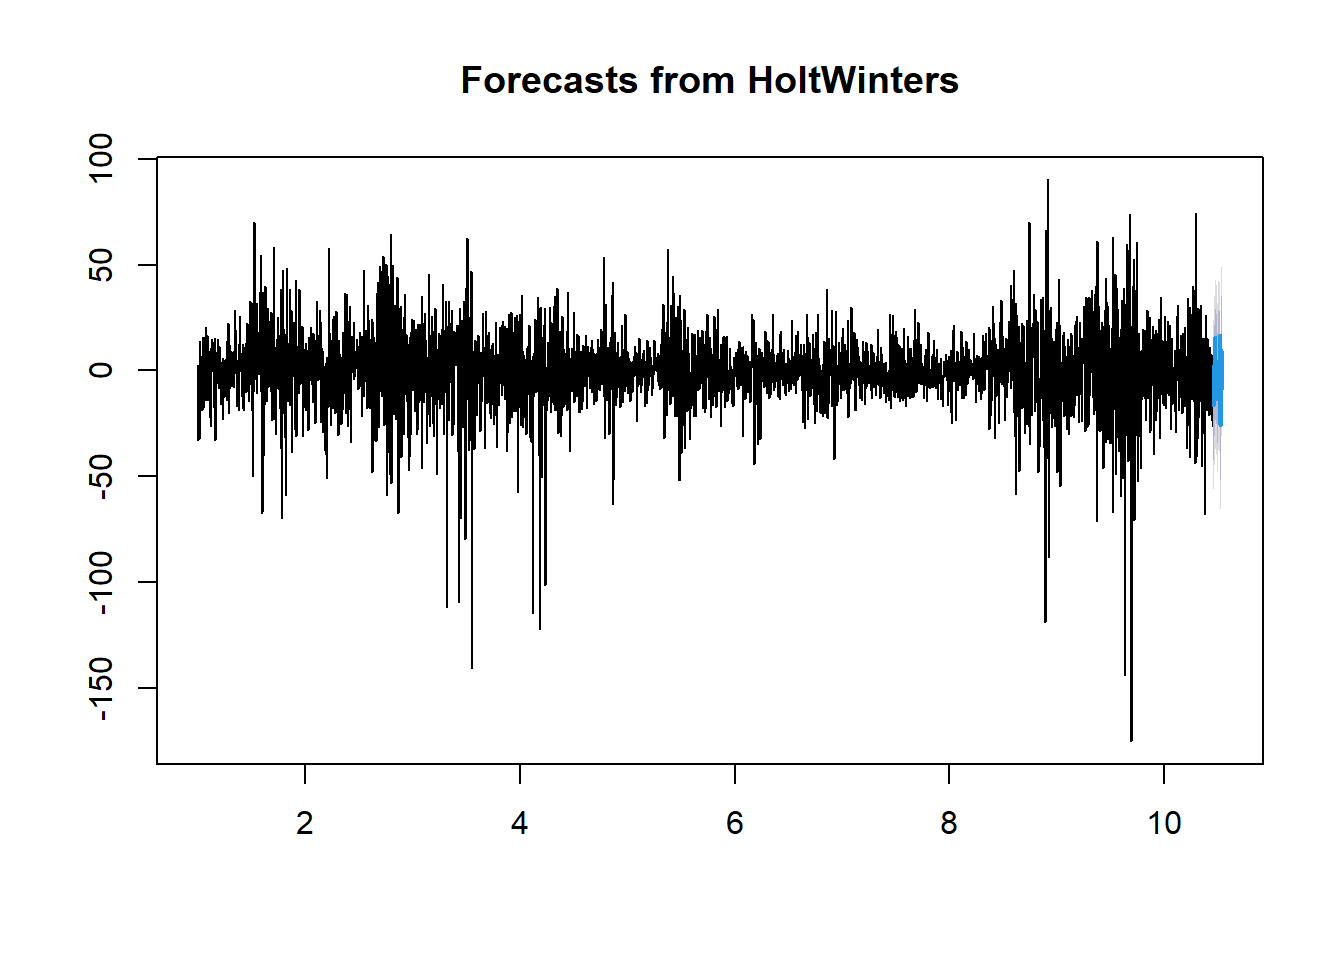
\includegraphics{bookdown-demo_files/figure-latex/unnamed-chunk-20-1.pdf}

\begin{Shaded}
\begin{Highlighting}[]
\CommentTok{\# Pronosticar los siguientes 30 días (o la cantidad que desees)}
\FunctionTok{library}\NormalTok{(forecast)}
\NormalTok{hw\_forecast }\OtherTok{\textless{}{-}} \FunctionTok{forecast}\NormalTok{(hw\_model, }\AttributeTok{h =} \DecValTok{30}\NormalTok{)  }\CommentTok{\# Cambia 30 por el número de periodos que quieras pronosticar}
\FunctionTok{plot}\NormalTok{(hw\_forecast)}
\end{Highlighting}
\end{Shaded}

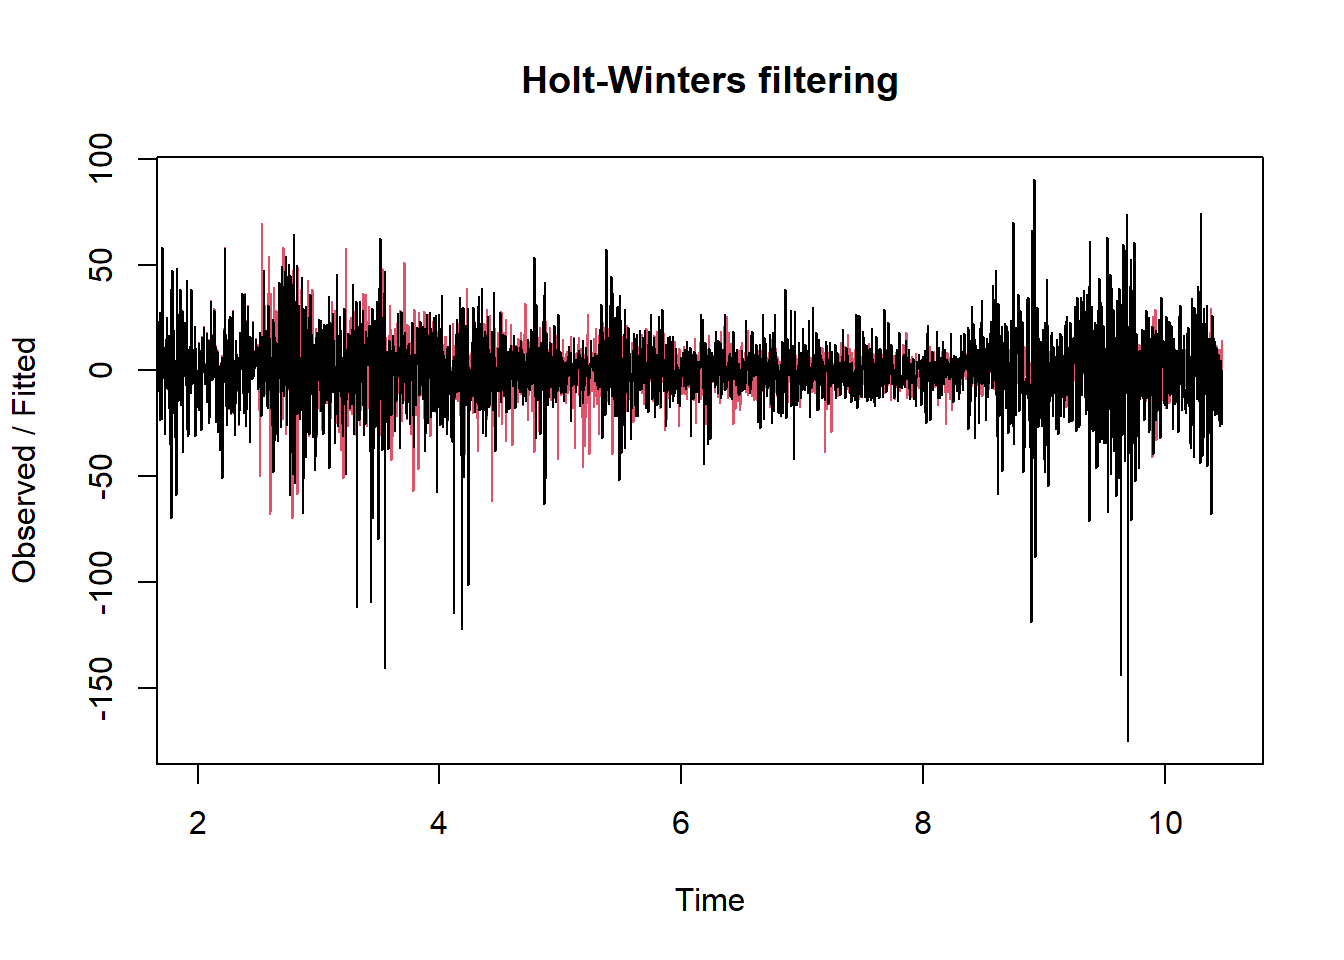
\includegraphics{bookdown-demo_files/figure-latex/unnamed-chunk-21-1.pdf}

\begin{Shaded}
\begin{Highlighting}[]
\CommentTok{\# Revisar detalles del modelo y del pronóstico}
\FunctionTok{summary}\NormalTok{(hw\_model)}
\end{Highlighting}
\end{Shaded}

\begin{verbatim}
##              Length Class  Mode     
## fitted       12348  mts    numeric  
## x             3452  ts     numeric  
## alpha            1  -none- numeric  
## beta             1  -none- numeric  
## gamma            1  -none- numeric  
## coefficients   367  -none- numeric  
## seasonal         1  -none- character
## SSE              1  -none- numeric  
## call             2  -none- call
\end{verbatim}

\begin{Shaded}
\begin{Highlighting}[]
\FunctionTok{summary}\NormalTok{(hw\_forecast)}
\end{Highlighting}
\end{Shaded}

\begin{verbatim}
## 
## Forecast method: HoltWinters
## 
## Model Information:
## Holt-Winters exponential smoothing with trend and additive seasonal component.
## 
## Call:
## HoltWinters(x = soybean_ts)
## 
## Smoothing parameters:
##  alpha: 0.001513595
##  beta : 0
##  gamma: 0.3523387
## 
## Coefficients:
##               [,1]
## a     -1.929391138
## b     -0.001484417
## s1     4.582162383
## s2     2.917054320
## s3    -2.792023886
## s4    16.438699482
## s5    10.324668487
## s6    17.926924350
## s7     5.229401015
## s8   -11.326377965
## s9     0.963002245
## s10    3.007431334
## s11    1.798317222
## s12   -3.367555137
## s13   -0.288966674
## s14   -6.256853382
## s15    0.468146356
## s16    6.237588050
## s17    4.798310102
## s18   -4.144225802
## s19   -9.696902544
## s20    3.720422996
## s21    6.916946502
## s22   -0.323101548
## s23   18.792492632
## s24  -23.815178035
## s25   11.560375345
## s26   -6.126604491
## s27   11.363620621
## s28    6.818268284
## s29   -6.403242763
## s30    1.183016479
## s31    0.671356135
## s32   18.851600512
## s33   10.311896291
## s34  -16.750753452
## s35    7.154940441
## s36   18.997617648
## s37   -4.232110804
## s38    2.587679523
## s39   10.740245891
## s40    5.347627847
## s41    8.698699935
## s42    3.632347595
## s43  -10.917325854
## s44   -1.966024311
## s45    0.948067100
## s46   10.231119777
## s47    4.127298154
## s48   -5.211077122
## s49   -6.615404268
## s50  -21.180146051
## s51   12.973504422
## s52    7.723456160
## s53   16.768126045
## s54   -0.163355807
## s55   -4.699983094
## s56  -18.563517056
## s57  -14.144309214
## s58  -12.700828126
## s59   15.057799618
## s60   17.042194147
## s61    7.282569696
## s62  -20.771751904
## s63    1.987600563
## s64    6.129687038
## s65  -52.312998249
## s66   14.410245702
## s67   -8.416780621
## s68   -9.268680523
## s69   -6.020895243
## s70   11.064892994
## s71    2.825000670
## s72   27.504347880
## s73   18.069057262
## s74   14.719539445
## s75    8.705219038
## s76  -16.209724754
## s77   -8.319567688
## s78   -1.276135074
## s79   30.522192082
## s80   10.203557698
## s81   -0.136192108
## s82   26.162721641
## s83   -1.440324386
## s84   12.807794895
## s85  -13.426041132
## s86  -60.788271125
## s87   -6.660617534
## s88   11.418984967
## s89    7.679685592
## s90   -9.997822602
## s91   14.116502278
## s92   19.211660994
## s93    0.539178182
## s94   -2.873923293
## s95   17.775781959
## s96  -28.214970933
## s97    0.776003611
## s98   -0.497434437
## s99   -5.872658545
## s100  12.762425533
## s101  -5.352988480
## s102 -10.681658678
## s103   0.421714157
## s104   0.427871448
## s105  38.625818330
## s106 -10.549033307
## s107  -7.761475630
## s108 -14.387806014
## s109  -2.771739765
## s110   9.087295651
## s111   2.484195187
## s112 -13.370816176
## s113   1.294512835
## s114  -5.527608642
## s115   0.146940645
## s116   7.023424623
## s117   6.310197846
## s118   4.266829113
## s119 -10.795176126
## s120  13.072370600
## s121   2.335212768
## s122   1.590108116
## s123  -7.780563459
## s124   4.557244385
## s125   0.889611758
## s126  10.300452874
## s127   1.838701772
## s128   3.100609200
## s129  -3.663511676
## s130   5.181658124
## s131  -1.532601854
## s132  -0.960802162
## s133   8.508378200
## s134   6.912061490
## s135 -20.934818384
## s136   1.535039770
## s137  -3.486978217
## s138   2.789103773
## s139  -5.993153107
## s140   8.960305939
## s141  11.068347504
## s142   3.115141118
## s143  -7.251313366
## s144   8.586302253
## s145   5.512433483
## s146   3.793838471
## s147  16.771853632
## s148  -9.348245985
## s149   2.781361605
## s150   3.403226487
## s151  -1.047832761
## s152  -5.578235778
## s153  -6.438040227
## s154  -1.972977675
## s155  -2.509062276
## s156  -9.725611917
## s157   1.843034329
## s158  -3.991155429
## s159 -17.638890136
## s160  18.932666612
## s161   9.981509005
## s162 -17.405684860
## s163   2.593087066
## s164  -1.240272512
## s165  -5.705074203
## s166  14.041020124
## s167   6.082258683
## s168  19.198665502
## s169  -8.552206193
## s170   8.121017409
## s171 -19.072117695
## s172   0.235352203
## s173   3.984638277
## s174  -2.587484896
## s175  13.185375964
## s176   3.124224196
## s177   1.129992687
## s178   0.336185546
## s179   4.946881486
## s180   3.275655434
## s181   3.584194592
## s182   4.032667680
## s183 -16.123356654
## s184  -7.698235874
## s185   0.770426333
## s186  15.049507138
## s187   5.621259981
## s188   3.003154305
## s189  -1.537679430
## s190   6.942001848
## s191  -4.635975724
## s192   2.954637074
## s193  -5.441290264
## s194   1.838159913
## s195  -0.438877219
## s196  -1.744332683
## s197  -6.970300846
## s198   4.699455343
## s199  15.668290510
## s200 -15.209805874
## s201   6.048468650
## s202  -2.666979611
## s203 -11.315066405
## s204  -1.706858378
## s205  -0.137737151
## s206   5.294759742
## s207  -1.727073232
## s208   8.471293098
## s209  -1.798925820
## s210  -0.484597124
## s211   3.591101328
## s212  -2.536255553
## s213  -3.398325492
## s214   1.013209649
## s215  -3.034840398
## s216  11.361005281
## s217  -1.560753569
## s218   2.504258743
## s219  -5.755239934
## s220  -4.765103319
## s221  -5.844821473
## s222   5.887393617
## s223   3.339453837
## s224  -0.124135110
## s225   9.127919804
## s226  -2.763851078
## s227  -1.387825854
## s228  -2.245018188
## s229  -0.737054785
## s230  -3.817434793
## s231   1.576819624
## s232  -9.765449979
## s233  -1.408391688
## s234  -7.982348074
## s235   6.657261602
## s236  -9.006840572
## s237  -5.460474313
## s238  -7.765921513
## s239   4.690360692
## s240   0.315751664
## s241   8.334506749
## s242   3.269035110
## s243   1.541180092
## s244  14.511981270
## s245  10.105630937
## s246   2.873948206
## s247  -5.067081849
## s248  -7.224419107
## s249   2.883684724
## s250   6.437547235
## s251   6.022852407
## s252  -1.275898252
## s253   1.216723124
## s254   8.014533133
## s255   2.403066271
## s256  -3.248248135
## s257  -6.253222843
## s258  -7.061377256
## s259 -10.354270330
## s260   0.737013910
## s261   2.304455115
## s262   0.597155785
## s263  13.009742256
## s264   7.515159848
## s265 -12.782093524
## s266   9.934012155
## s267  -2.162980361
## s268   9.096788779
## s269   4.611906907
## s270  -2.925270933
## s271  -8.608644113
## s272  -0.669661523
## s273  -6.386286085
## s274 -16.515971667
## s275  -7.903660629
## s276  -5.251559017
## s277   4.151109422
## s278 -13.041123426
## s279  11.841886870
## s280  -1.642324074
## s281   5.538959377
## s282   4.356173173
## s283  -0.131828463
## s284  -8.519052220
## s285  -2.380294085
## s286  14.837057715
## s287  11.012540633
## s288  -0.018949025
## s289   3.965308404
## s290   9.544823454
## s291   3.826160159
## s292  17.732556175
## s293  -4.096190452
## s294  10.414114179
## s295 -10.436449250
## s296  15.541873429
## s297  18.795860143
## s298  13.617378581
## s299  14.109554993
## s300  -6.234603325
## s301   4.097378093
## s302   5.136980691
## s303  -6.216264765
## s304 -10.993671497
## s305   5.365792494
## s306  25.677948405
## s307   0.748032229
## s308   2.406747444
## s309   2.127176810
## s310 -15.279212965
## s311   7.757276904
## s312   8.713054071
## s313  -2.955336663
## s314  13.109781815
## s315  -0.089637039
## s316   0.910850818
## s317  13.526850902
## s318   4.027480269
## s319   2.853394948
## s320   9.379620328
## s321  15.572132827
## s322  -1.256885365
## s323  20.730227438
## s324  -8.438975318
## s325 -12.888249928
## s326 -12.814128195
## s327  -2.428184949
## s328   2.468134704
## s329   3.652568673
## s330  10.927992549
## s331  -1.278166371
## s332  18.902577548
## s333   1.144003263
## s334 -24.383756339
## s335  10.715309724
## s336  17.168361718
## s337 -26.967672571
## s338   2.344103368
## s339  -1.776835237
## s340   8.714972888
## s341  10.777991068
## s342  -9.784349003
## s343   5.569313202
## s344   1.369166623
## s345   8.354150140
## s346  -1.112880071
## s347  -5.066524267
## s348   6.395679771
## s349  -4.590388609
## s350   6.224730075
## s351  -0.634782605
## s352  13.485164749
## s353 -12.946619992
## s354   5.780986256
## s355  -9.225156092
## s356  -8.091836858
## s357   6.228798507
## s358  -6.862548862
## s359  -6.884365352
## s360  -1.789971174
## s361   7.975252378
## s362   2.221258945
## s363  -0.977014208
## s364   9.358837965
## s365  -8.034359349
## 
## Error measures:
##                     ME     RMSE      MAE MPE MAPE      MASE       ACF1
## Training set 0.3675777 20.36142 14.07497 NaN  Inf 0.7995699 0.02160829
## 
## Forecasts:
##          Point Forecast      Lo 80     Hi 80     Lo 95    Hi 95
## 10.46027      2.6512868 -23.442894 28.745467 -37.25632 42.55889
## 10.46301      0.9846943 -25.109516 27.078905 -38.92296 40.89235
## 10.46575     -4.7258683 -30.820109 21.368372 -44.63357 35.18183
## 10.46849     14.5033707 -11.590900 40.597641 -25.40437 54.41111
## 10.47123      8.3878553 -17.706445 34.482155 -31.51993 48.29564
## 10.47397     15.9886267 -10.105703 42.082957 -23.91921 55.89646
## 10.47671      3.2896190 -22.804741 29.383979 -36.61826 43.19750
## 10.47945    -13.2676444 -39.362034 12.826745 -53.17557 26.64028
## 10.48219     -0.9797486 -27.074168 25.114671 -40.88772 38.92822
## 10.48493      1.0631960 -25.031254 27.157646 -38.84482 40.97121
## 10.48767     -0.1474025 -26.241882 25.947077 -40.05547 39.76066
## 10.49041     -5.3147593 -31.409269 20.779750 -45.22287 34.59335
## 10.49315     -2.2376552 -28.332195 23.856884 -42.14581 37.67050
## 10.49589     -8.2070264 -34.301596 17.887543 -48.11523 31.70117
## 10.49863     -1.4835110 -27.578110 24.611088 -41.39176 38.42473
## 10.50137      4.2844462 -21.810183 30.379075 -35.62384 44.19274
## 10.50411      2.8436839 -23.250975 28.938343 -37.06465 42.75202
## 10.50685     -6.1003364 -32.195025 19.994352 -46.00872 33.80805
## 10.50959    -11.6544976 -37.749216 14.440221 -51.56293 28.25393
## 10.51233      1.7613435 -24.333405 27.856092 -38.14713 41.66982
## 10.51507      4.9563826 -21.138396 31.051161 -34.95214 44.86490
## 10.51781     -2.2851498 -28.379958 23.809658 -42.19372 37.62342
## 10.52055     16.8289599  -9.265878 42.923798 -23.07965 56.73757
## 10.52329    -25.7801952 -51.875063  0.314673 -65.68885 14.12846
## 10.52603      9.5938738 -16.501024 35.688772 -30.31483 49.50258
## 10.52877     -8.0945905 -34.189518 18.000337 -48.00334 31.81416
## 10.53151      9.3941502 -16.700808 35.489108 -30.51464 49.30294
## 10.53425      4.8473135 -21.247674 30.942301 -35.06153 44.75615
## 10.53699     -8.3756820 -34.470700 17.719336 -48.28457 31.53320
## 10.53973     -0.7909072 -26.885955 25.304140 -40.69984 39.11802
\end{verbatim}

\hypertarget{arima}{%
\chapter{ARIMA}\label{arima}}

ARIMA es como un método o herramienta que nos ayuda a entender y prever cómo se comportará una secuencia de números en el futuro, basándose en cómo se ha comportado en el pasado.

\begin{Shaded}
\begin{Highlighting}[]
\NormalTok{modelo}\OtherTok{\textless{}{-}}\FunctionTok{auto.arima}\NormalTok{(soybean\_ts)}
\NormalTok{modelo}
\end{Highlighting}
\end{Shaded}

\begin{verbatim}
## Series: soybean_ts 
## ARIMA(0,0,0) with zero mean 
## 
## sigma^2 = 314.9:  log likelihood = -14826.36
## AIC=29654.72   AICc=29654.72   BIC=29660.86
\end{verbatim}

Conclusión:

El resultado de auto.arima() elige un modelo ARIMA(0,0,0) con media cero,indica según el análisis que no hay patrones, ritmos, ni tendencias claras en los datos de la serie de tiempo del precio del aceite de soya.

Los valores de la serie de tiempo del precio delaceite de soya son como un conjunto de números aleatorios, o ``ruido blanco'', sin conexión aparente entre ellos. En otras palabras, cada punto de datos es independiente de los otros y no está influenciado por los valores pasados en la serie.

\begin{Shaded}
\begin{Highlighting}[]
\FunctionTok{length}\NormalTok{(soybean\_ts)}
\end{Highlighting}
\end{Shaded}

\begin{verbatim}
## [1] 3452
\end{verbatim}

\begin{Shaded}
\begin{Highlighting}[]
\FunctionTok{sum}\NormalTok{(}\FunctionTok{is.na}\NormalTok{(soybean\_ts))}
\end{Highlighting}
\end{Shaded}

\begin{verbatim}
## [1] 0
\end{verbatim}

\begin{Shaded}
\begin{Highlighting}[]
\FunctionTok{class}\NormalTok{(soybean\_ts)}
\end{Highlighting}
\end{Shaded}

\begin{verbatim}
## [1] "ts"
\end{verbatim}

\begin{Shaded}
\begin{Highlighting}[]
\FunctionTok{sum}\NormalTok{(}\FunctionTok{is.na}\NormalTok{(soybean\_ts) }\SpecialCharTok{|} \FunctionTok{is.infinite}\NormalTok{(soybean\_ts))}
\end{Highlighting}
\end{Shaded}

\begin{verbatim}
## [1] 0
\end{verbatim}

\begin{Shaded}
\begin{Highlighting}[]
\CommentTok{\# Instalar el paquete changepoint}
\CommentTok{\#install.packages("changepoint")}

\CommentTok{\# Cargar el paquete changepoint}
\FunctionTok{library}\NormalTok{(changepoint)}
\end{Highlighting}
\end{Shaded}

\begin{verbatim}
## Warning: package 'changepoint' was built under R version 4.2.3
\end{verbatim}

\begin{verbatim}
## Successfully loaded changepoint package version 2.2.4
##  See NEWS for details of changes.
\end{verbatim}

\begin{Shaded}
\begin{Highlighting}[]
\NormalTok{mval\_soybean }\OtherTok{\textless{}{-}} \FunctionTok{cpt.mean}\NormalTok{(}\FunctionTok{as.numeric}\NormalTok{(soybean\_ts), }\AttributeTok{method =} \StringTok{"AMOC"}\NormalTok{)}
\FunctionTok{cpts}\NormalTok{(mval\_soybean)}
\end{Highlighting}
\end{Shaded}

\begin{verbatim}
## [1] 3410
\end{verbatim}

\begin{Shaded}
\begin{Highlighting}[]
\CommentTok{\# Plot de la serie de tiempo}
\FunctionTok{plot}\NormalTok{(soybean\_ts, }\AttributeTok{type=}\StringTok{\textquotesingle{}l\textquotesingle{}}\NormalTok{, }\AttributeTok{main=}\StringTok{\textquotesingle{}Serie de Tiempo con Punto de Cambio\textquotesingle{}}\NormalTok{, }\AttributeTok{ylab=}\StringTok{\textquotesingle{}Valor\textquotesingle{}}\NormalTok{, }\AttributeTok{xlab=}\StringTok{\textquotesingle{}Tiempo\textquotesingle{}}\NormalTok{)}

\CommentTok{\# Añadir una línea vertical en el punto de cambio}
\FunctionTok{abline}\NormalTok{(}\AttributeTok{v=}\DecValTok{3410}\NormalTok{, }\AttributeTok{col=}\StringTok{\textquotesingle{}red\textquotesingle{}}\NormalTok{, }\AttributeTok{lty=}\DecValTok{2}\NormalTok{, }\AttributeTok{lwd=}\DecValTok{2}\NormalTok{)}

\CommentTok{\# Añadir una leyenda}
\FunctionTok{legend}\NormalTok{(}\StringTok{"topright"}\NormalTok{, }\AttributeTok{legend=}\StringTok{"Punto de Cambio"}\NormalTok{, }\AttributeTok{col=}\StringTok{"red"}\NormalTok{, }\AttributeTok{lty=}\DecValTok{2}\NormalTok{, }\AttributeTok{lwd=}\DecValTok{2}\NormalTok{)}
\end{Highlighting}
\end{Shaded}

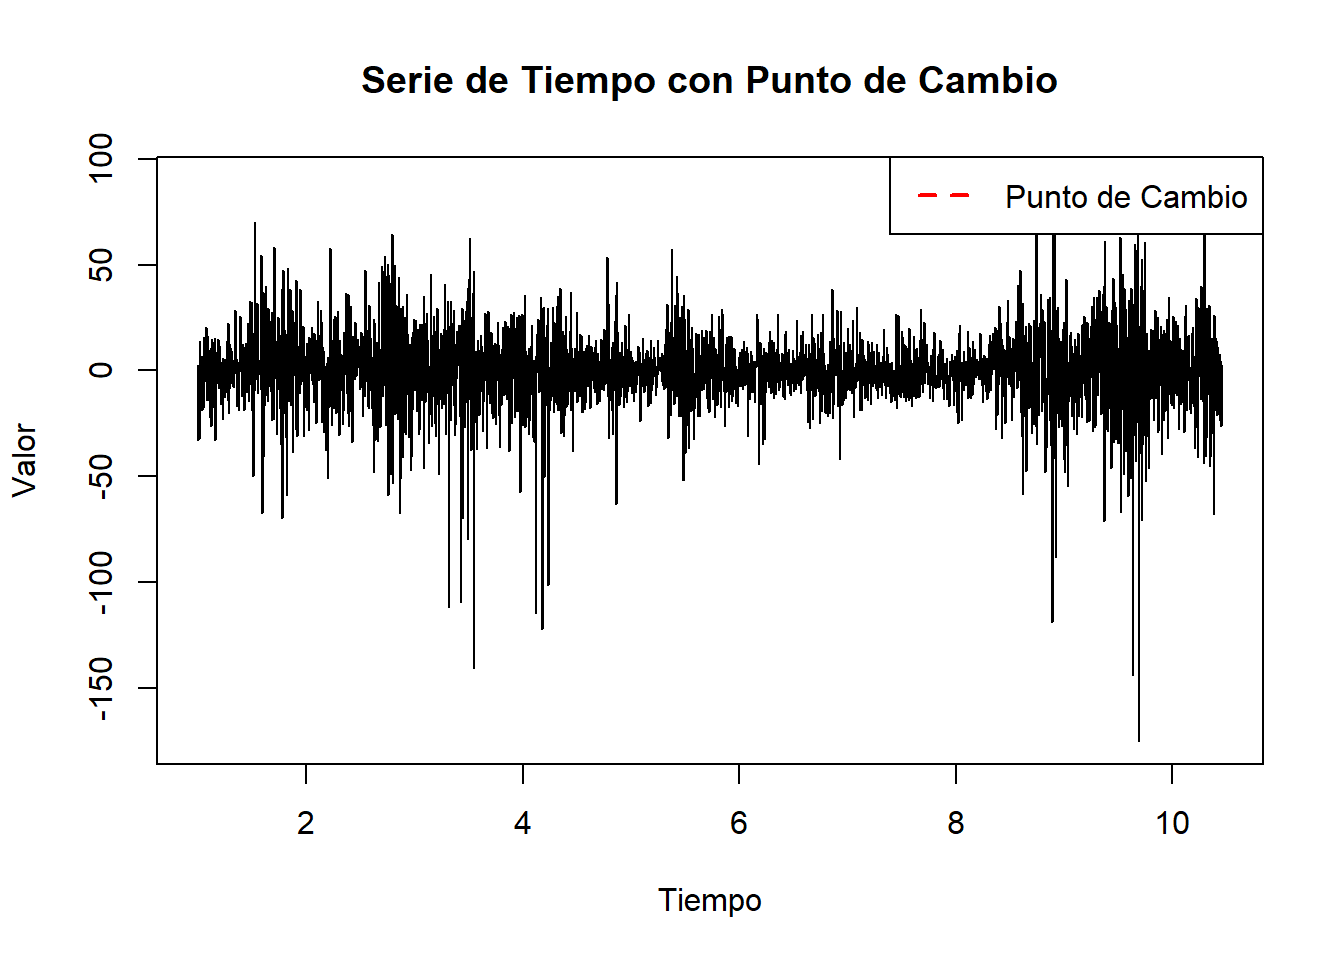
\includegraphics{bookdown-demo_files/figure-latex/unnamed-chunk-26-1.pdf}

\begin{Shaded}
\begin{Highlighting}[]
\NormalTok{pred}\OtherTok{\textless{}{-}}\FunctionTok{forecast}\NormalTok{(soybean\_ts,}\AttributeTok{h=}\DecValTok{12}\NormalTok{)}
\NormalTok{pred}
\end{Highlighting}
\end{Shaded}

\begin{verbatim}
##          Point Forecast     Lo 80    Hi 80     Lo 95    Hi 95
## 10.46027       1.705264 -18.49799 21.90851 -29.19294 32.60347
## 10.46301      -1.864569 -22.06782 18.33868 -32.76277 29.03364
## 10.46575      -8.091969 -28.29522 12.11128 -38.99017 22.80624
## 10.46849       9.907042 -10.29621 30.11029 -20.99116 40.80525
## 10.47123       9.176571 -11.02668 29.37982 -21.72163 40.07478
## 10.47397       9.721777 -10.48147 29.92503 -21.17643 40.61998
## 10.47671       6.436872 -13.76638 26.64012 -24.46133 37.33508
## 10.47945      -7.249053 -27.45230 12.95420 -38.14726 23.64915
## 10.48219      -4.373007 -24.57626 15.83024 -35.27121 26.52520
## 10.48493       1.090572 -19.11268 21.29382 -29.80763 31.98878
## 10.48767      -6.707186 -26.91044 13.49607 -37.60539 24.19102
## 10.49041       1.096394 -19.10686 21.29965 -29.80181 31.99460
\end{verbatim}

\begin{Shaded}
\begin{Highlighting}[]
\FunctionTok{plot}\NormalTok{(pred, }\AttributeTok{main=}\StringTok{" "}\NormalTok{, }\AttributeTok{ylab=}\StringTok{"valor"}\NormalTok{, }\AttributeTok{col=}\StringTok{"deepskyblue"}\NormalTok{, }\AttributeTok{xlab=}\StringTok{"Tiempo"}\NormalTok{)}
\FunctionTok{title}\NormalTok{(}\AttributeTok{main=}\StringTok{"Predicción DIF Precios del aceite de soya"}\NormalTok{)}
\end{Highlighting}
\end{Shaded}

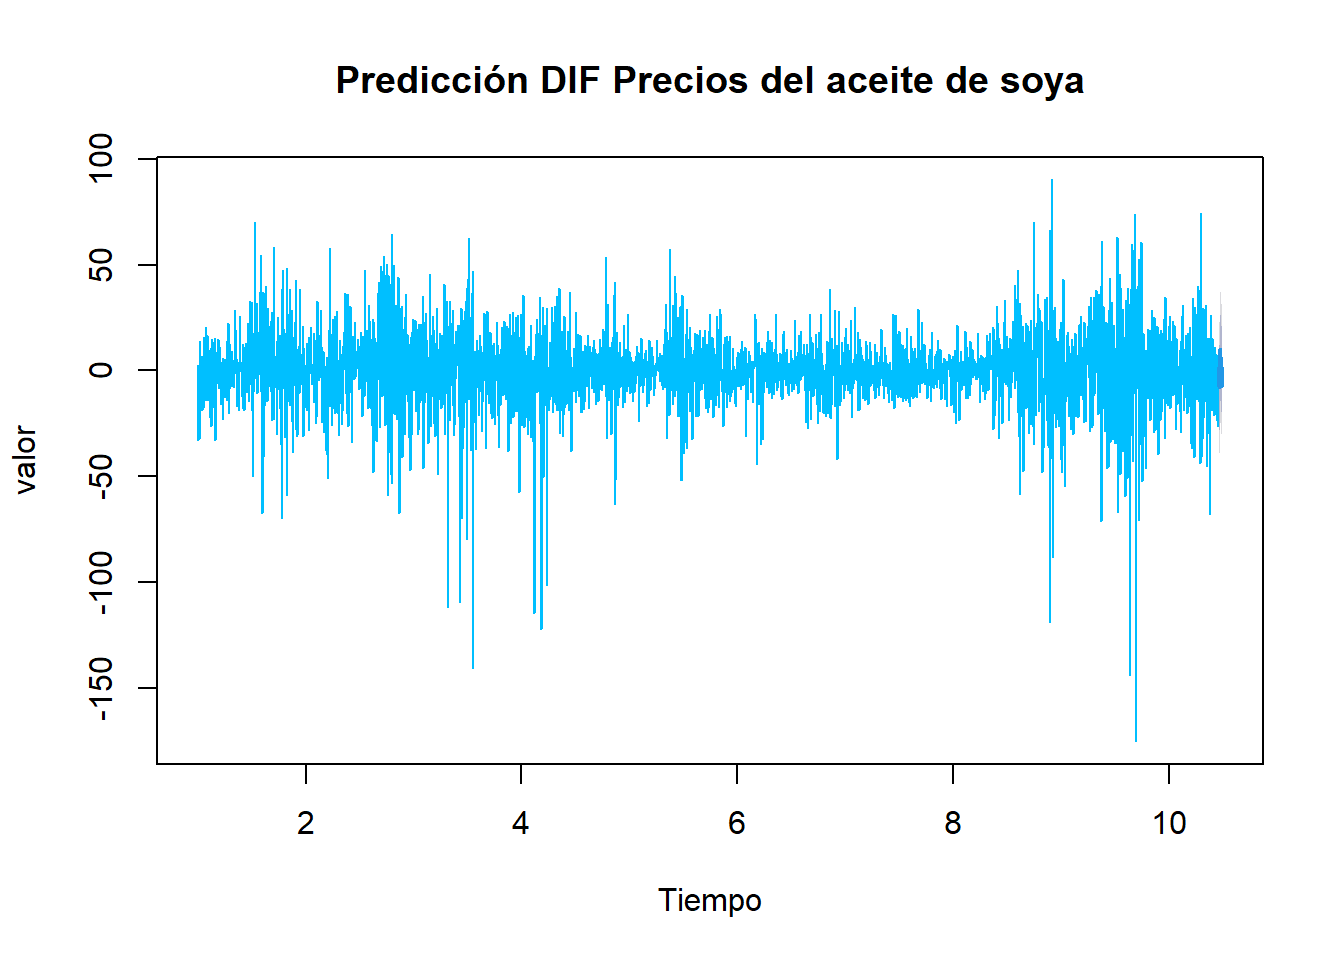
\includegraphics{bookdown-demo_files/figure-latex/unnamed-chunk-28-1.pdf}

\hypertarget{prophet}{%
\chapter{Prophet}\label{prophet}}

Prophet es especialmente útil para series de tiempo que tienen patrones estacionales fuertes y varios puntos de inflexión o ``cambios de tendencia''. Fue diseñado para manejar datos diarios con al menos un año de historia y se espera que funcione bien con datos que tienen patrones estacionales y fechas festivas.

\begin{Shaded}
\begin{Highlighting}[]
\CommentTok{\# install.packages("prophet")}
\FunctionTok{library}\NormalTok{(prophet)}
\end{Highlighting}
\end{Shaded}

\begin{verbatim}
## Warning: package 'prophet' was built under R version 4.2.3
\end{verbatim}

\begin{verbatim}
## Loading required package: Rcpp
\end{verbatim}

\begin{verbatim}
## Warning: package 'Rcpp' was built under R version 4.2.3
\end{verbatim}

\begin{verbatim}
## Loading required package: rlang
\end{verbatim}

\begin{verbatim}
## Warning: package 'rlang' was built under R version 4.2.3
\end{verbatim}

\begin{Shaded}
\begin{Highlighting}[]
\CommentTok{\# Acceder a la columna "ZS.F.Close" en soybean\_xts}
\NormalTok{close\_prices }\OtherTok{\textless{}{-}}\NormalTok{ soybean\_xts[, }\StringTok{"ZS.F.Close"}\NormalTok{]}

\CommentTok{\# Extrae las fechas}
\NormalTok{dates }\OtherTok{\textless{}{-}} \FunctionTok{index}\NormalTok{(soybean\_xts)}

\CommentTok{\# Crea el dataframe}
\NormalTok{soybean\_df }\OtherTok{\textless{}{-}} \FunctionTok{data.frame}\NormalTok{(}\AttributeTok{ds =} \FunctionTok{as.Date}\NormalTok{(dates), }\AttributeTok{y =} \FunctionTok{as.numeric}\NormalTok{(close\_prices))}
\end{Highlighting}
\end{Shaded}

\begin{Shaded}
\begin{Highlighting}[]
\FunctionTok{head}\NormalTok{(soybean\_df)}
\end{Highlighting}
\end{Shaded}

\begin{verbatim}
##           ds       y
## 1 2010-01-04 1049.50
## 2 2010-01-05 1052.25
## 3 2010-01-06 1050.50
## 4 2010-01-07 1017.75
## 5 2010-01-08 1013.00
## 6 2010-01-11 1001.75
\end{verbatim}

\begin{Shaded}
\begin{Highlighting}[]
\NormalTok{m }\OtherTok{\textless{}{-}} \FunctionTok{prophet}\NormalTok{(soybean\_df)}
\end{Highlighting}
\end{Shaded}

\begin{verbatim}
## Disabling daily seasonality. Run prophet with daily.seasonality=TRUE to override this.
\end{verbatim}

\begin{Shaded}
\begin{Highlighting}[]
\NormalTok{future }\OtherTok{\textless{}{-}} \FunctionTok{make\_future\_dataframe}\NormalTok{(m, }\AttributeTok{periods =} \DecValTok{365}\NormalTok{) }
\NormalTok{forecast }\OtherTok{\textless{}{-}} \FunctionTok{predict}\NormalTok{(m, future)}
\end{Highlighting}
\end{Shaded}

\begin{Shaded}
\begin{Highlighting}[]
\FunctionTok{plot}\NormalTok{(m, forecast)}
\end{Highlighting}
\end{Shaded}

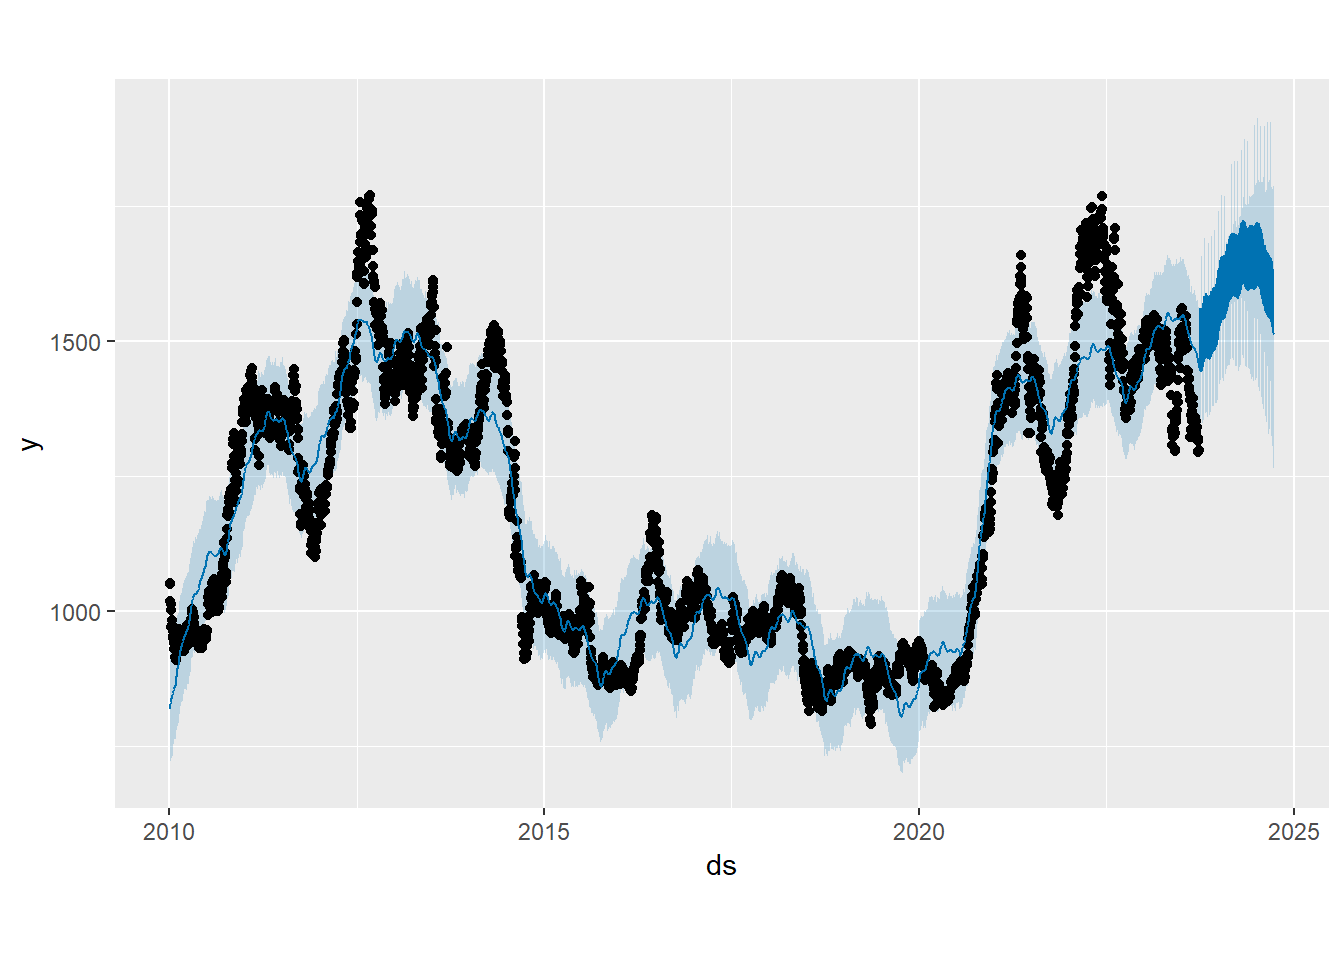
\includegraphics{bookdown-demo_files/figure-latex/unnamed-chunk-33-1.pdf}

\begin{Shaded}
\begin{Highlighting}[]
\FunctionTok{prophet\_plot\_components}\NormalTok{(m, forecast)}
\end{Highlighting}
\end{Shaded}

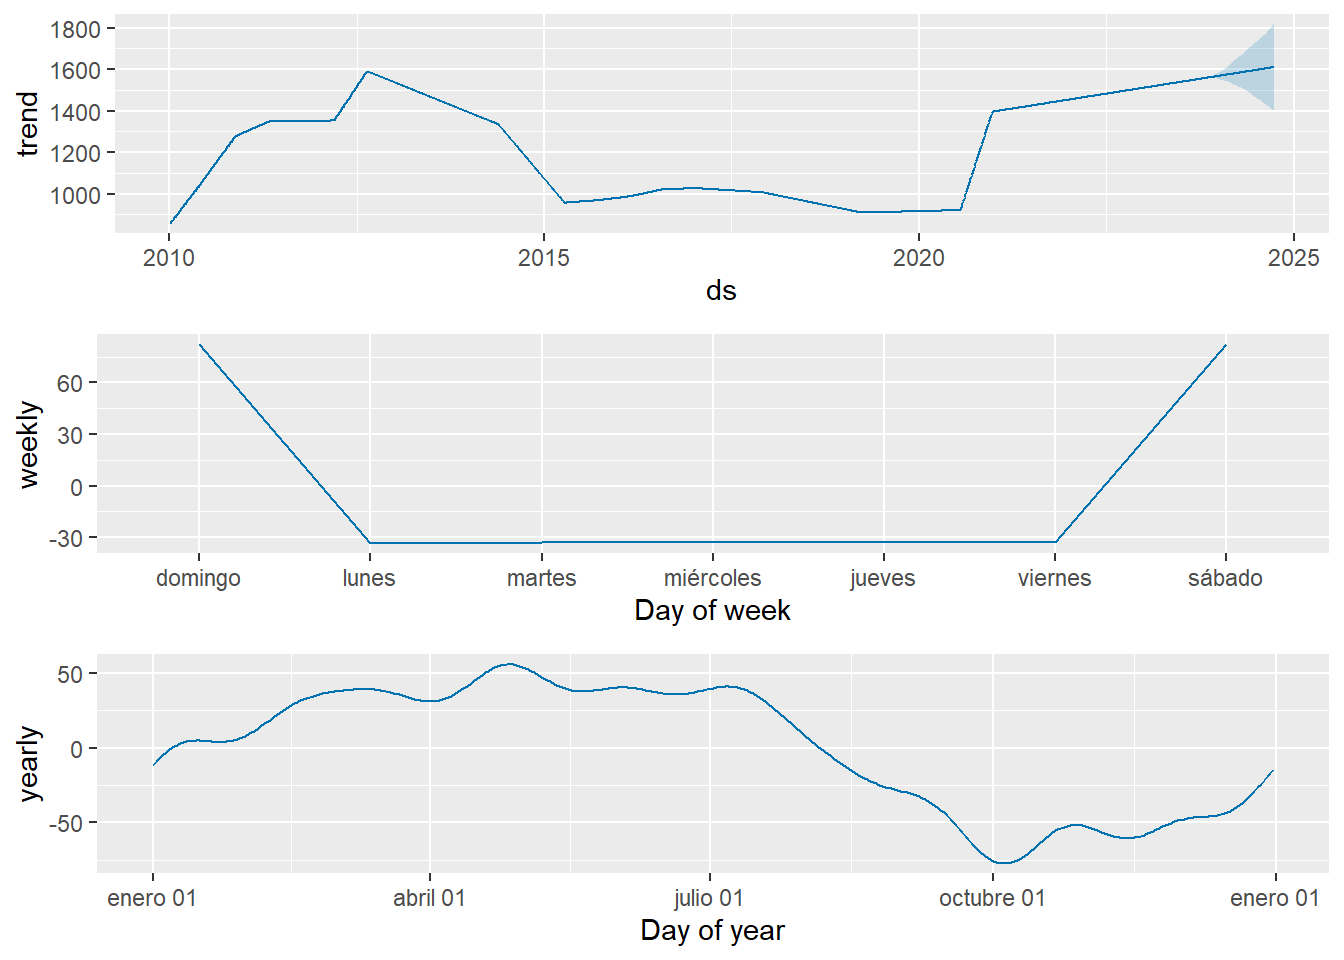
\includegraphics{bookdown-demo_files/figure-latex/unnamed-chunk-33-2.pdf}

\begin{Shaded}
\begin{Highlighting}[]
\FunctionTok{library}\NormalTok{(ggplot2)}

\CommentTok{\# Extraer datos del pronóstico}
\CommentTok{\# forecast\_data \textless{}{-} data.frame(}
\CommentTok{\#  ds = forecast$ds, }
\CommentTok{\#  yhat = forecast$yhat, }
\CommentTok{\#  yhat\_lower = forecast$yhat\_lower, }
\CommentTok{\#  yhat\_upper = forecast$yhat\_upper}
\CommentTok{\#)}

\CommentTok{\# Datos reales}
\CommentTok{\#actual\_data \textless{}{-} data.frame(ds = m$history$ds, y = m$history$y)}

\CommentTok{\# Crear el gráfico con ggplot2}
\CommentTok{\#p \textless{}{-} ggplot() +}
  \CommentTok{\# Intervalo de confianza}
\CommentTok{\#  geom\_ribbon(data = forecast\_data, aes(x = ds, ymin = yhat\_lower, ymax = \#yhat\_upper, fill = "Intervalo de Confianza"), alpha = 0.4, inherit.aes = FALSE) +}
  \CommentTok{\# Línea de pronóstico}
\CommentTok{\#  geom\_line(data = forecast\_data, aes(x = ds, y = yhat, color = "Pronóstico"), size = 1, inherit.aes = FALSE) + }
  \CommentTok{\# Datos reales}
\CommentTok{\#  geom\_point(data = actual\_data, aes(x = ds, y = y, color = "Datos Reales"), size \#= 2, inherit.aes = FALSE) +}
  \CommentTok{\# Tema y etiquetas}
\CommentTok{\#  theme\_minimal() +}
\CommentTok{\#  labs(}
\CommentTok{\#    title = "Pronóstico del Precio del Aceite de Soya",}
\CommentTok{\#    x = "Fecha",}
\CommentTok{\#   y = "Precio"}
\CommentTok{\#  ) +}
\CommentTok{\#  scale\_fill\_manual(}
    \CommentTok{\#name = "Leyenda",}
\CommentTok{\#    values = c("Intervalo de Confianza" = "lightblue"),}
\CommentTok{\#    labels = c("Intervalo de Confianza")}
\CommentTok{\#  ) +}
\CommentTok{\#  scale\_color\_manual(}
    \CommentTok{\#name = "Leyenda",}
\CommentTok{\#    values = c("Datos Reales" = "\#D55E00", "Pronóstico" = "\#0072B2"),}
\CommentTok{\#    labels = c("Datos Reales", "Pronóstico")}
\CommentTok{\#  ) +}
\CommentTok{\#  theme(legend.position = "bottom")}

\CommentTok{\# Mostrar gráfico}
\CommentTok{\#print(p)}
\end{Highlighting}
\end{Shaded}

\begin{Shaded}
\begin{Highlighting}[]
\CommentTok{\# library(ggplot2)}

\CommentTok{\# Extraer componentes del pronóstico}
\CommentTok{\# components \textless{}{-} prophet\_plot\_components(m, forecast)}

\CommentTok{\# Convertir el objeto básico de Prophet a ggplot}
\CommentTok{\# p\_components \textless{}{-} ggplot() +}
\CommentTok{\#  geom\_line(data = components$data$yearly, aes(x = ds, y = y, color = "Componente \# Anual"), size = 1) +}
\CommentTok{\#  geom\_line(data = components$data$weekly, aes(x = ds, y = y, color = "Componente \# Semanal"), size = 1) +}
\CommentTok{\#  geom\_line(data = components$data$daily, aes(x = ds, y = y, color = "Componente \# Diario"), size = 1) +}
\CommentTok{\#  geom\_line(data = components$data$holidays, aes(x = ds, y = y, color = "Días \# \# Festivos"), size = 1) +}
\CommentTok{\#  theme\_minimal() +}
\CommentTok{\#  labs(}
\CommentTok{\#    title = "Componentes del Pronóstico",}
\CommentTok{\#    x = "Fecha",}
\CommentTok{\#    y = "Valor"}
\CommentTok{\#  ) +}
\CommentTok{\#  scale\_color\_manual(}
\CommentTok{\#    name = "Leyenda",}
\CommentTok{\#    values = c("Componente Anual" = "blue", "Componente Semanal" = "green", \#"Componente Diario" = "red", "Días Festivos" = "orange")}
\CommentTok{\#  ) +}
\CommentTok{\#  theme(legend.position = "bottom")}

\CommentTok{\# Mostrar gráfico de componentes}
\CommentTok{\#print(p\_components)}
\end{Highlighting}
\end{Shaded}

Conclusión: Se toman datos de la serie de tiempo histórica del precio del aceite de soya, creamos un modelo de pronóstico con Prophet, y se produce pronósticos para 365 días adicionales y luego visualiza esos pronósticos y sus componentes.

Si es viable la justificación para la variable en serie de tiempo vista como una regresión y prophet permite la incorporación de variables exógenas a través de los regresores e identifica automáticamente las estacionalidades diarias, semanales y anuales en los datos. También captura las tendencias a lo largo del tiempo y permite puntos de cambio en la tendencia.

\hypertarget{elman}{%
\chapter{Elman}\label{elman}}

La red Elman es una red neuronal recurrente, lo que significa que tiene conexiones que retroceden en el tiempo. Estas conexiones permiten a la red ``recordar'' entradas anteriores, lo que puede ser útil al trabajar con series temporales.

\begin{Shaded}
\begin{Highlighting}[]
\CommentTok{\# Cargar los paquetes necesarios}
\CommentTok{\# install.packages("neuralnet")}
\CommentTok{\# install.packages("xts")}
\FunctionTok{library}\NormalTok{(neuralnet)}
\end{Highlighting}
\end{Shaded}

\begin{verbatim}
## Warning: package 'neuralnet' was built under R version 4.2.3
\end{verbatim}

\begin{Shaded}
\begin{Highlighting}[]
\FunctionTok{library}\NormalTok{(xts)}

\CommentTok{\# Asumimos que soybean\_xts ya está cargado en el entorno}
\CommentTok{\# Acceder a la columna de cierre}
\NormalTok{data }\OtherTok{\textless{}{-}} \FunctionTok{data.frame}\NormalTok{(}\AttributeTok{ZS.F.Close =} \FunctionTok{as.vector}\NormalTok{(soybean\_xts[, }\StringTok{"ZS.F.Close"}\NormalTok{]))}

\CommentTok{\# Crear un retraso (lag) para las series temporales (esto es importante para las redes recurrentes)}
\NormalTok{data}\SpecialCharTok{$}\NormalTok{lag\_close }\OtherTok{\textless{}{-}} \FunctionTok{c}\NormalTok{(}\ConstantTok{NA}\NormalTok{, }\FunctionTok{head}\NormalTok{(data}\SpecialCharTok{$}\NormalTok{ZS.F.Close, }\SpecialCharTok{{-}}\DecValTok{1}\NormalTok{))}

\CommentTok{\# Eliminar la primera fila, ya que tendrá NA por el retraso}
\NormalTok{data }\OtherTok{\textless{}{-}}\NormalTok{ data[}\SpecialCharTok{{-}}\DecValTok{1}\NormalTok{,]}

\CommentTok{\# Dividir los datos en conjuntos de entrenamiento y prueba}
\NormalTok{train\_indices }\OtherTok{\textless{}{-}} \DecValTok{1}\SpecialCharTok{:}\NormalTok{(}\FunctionTok{nrow}\NormalTok{(data) }\SpecialCharTok{*} \FloatTok{0.8}\NormalTok{)}
\NormalTok{train\_data }\OtherTok{\textless{}{-}}\NormalTok{ data[train\_indices,]}
\NormalTok{test\_data }\OtherTok{\textless{}{-}}\NormalTok{ data[}\SpecialCharTok{{-}}\NormalTok{train\_indices,]}

\CommentTok{\# Normalizar los datos}
\NormalTok{maxs }\OtherTok{\textless{}{-}} \FunctionTok{apply}\NormalTok{(train\_data, }\DecValTok{2}\NormalTok{, max)}
\NormalTok{mins }\OtherTok{\textless{}{-}} \FunctionTok{apply}\NormalTok{(train\_data, }\DecValTok{2}\NormalTok{, min)}
\NormalTok{train\_data\_norm }\OtherTok{\textless{}{-}} \FunctionTok{as.data.frame}\NormalTok{(}\FunctionTok{scale}\NormalTok{(train\_data, }\AttributeTok{center=}\NormalTok{mins, }\AttributeTok{scale=}\NormalTok{maxs}\SpecialCharTok{{-}}\NormalTok{mins))}
\NormalTok{test\_data\_norm }\OtherTok{\textless{}{-}} \FunctionTok{as.data.frame}\NormalTok{(}\FunctionTok{scale}\NormalTok{(test\_data, }\AttributeTok{center=}\NormalTok{mins, }\AttributeTok{scale=}\NormalTok{maxs}\SpecialCharTok{{-}}\NormalTok{mins))}

\CommentTok{\# Entrenar una red Elman }
\CommentTok{\# Aquí estamos prediciendo ZS.F.Close usando el valor anterior (lag\_close) como entrada}
\FunctionTok{set.seed}\NormalTok{(}\DecValTok{123}\NormalTok{)}
\NormalTok{nn }\OtherTok{\textless{}{-}} \FunctionTok{neuralnet}\NormalTok{(ZS.F.Close }\SpecialCharTok{\textasciitilde{}}\NormalTok{ lag\_close, }\AttributeTok{data=}\NormalTok{train\_data\_norm, }\AttributeTok{hidden=}\DecValTok{5}\NormalTok{, }\AttributeTok{algorithm=}\StringTok{"rprop+"}\NormalTok{, }\AttributeTok{linear.output=}\ConstantTok{TRUE}\NormalTok{, }\AttributeTok{likelihood=}\ConstantTok{TRUE}\NormalTok{)}

\CommentTok{\# Hacer predicciones}
\NormalTok{test\_data\_for\_pred }\OtherTok{\textless{}{-}} \FunctionTok{data.frame}\NormalTok{(}\AttributeTok{lag\_close =}\NormalTok{ test\_data\_norm}\SpecialCharTok{$}\NormalTok{lag\_close)}
\NormalTok{predicted\_norm }\OtherTok{\textless{}{-}} \FunctionTok{compute}\NormalTok{(nn, test\_data\_for\_pred)}

\CommentTok{\# Des{-}normalizar las predicciones}
\NormalTok{predicted }\OtherTok{\textless{}{-}}\NormalTok{ (predicted\_norm}\SpecialCharTok{$}\NormalTok{net.result }\SpecialCharTok{*}\NormalTok{ (maxs[}\DecValTok{1}\NormalTok{] }\SpecialCharTok{{-}}\NormalTok{ mins[}\DecValTok{1}\NormalTok{])) }\SpecialCharTok{+}\NormalTok{ mins[}\DecValTok{1}\NormalTok{]}

\CommentTok{\# Comparar las predicciones con los datos reales}
\FunctionTok{plot}\NormalTok{(test\_data}\SpecialCharTok{$}\NormalTok{ZS.F.Close, }\AttributeTok{type=}\StringTok{"l"}\NormalTok{, }\AttributeTok{col=}\StringTok{"blue"}\NormalTok{)}
\FunctionTok{lines}\NormalTok{(predicted, }\AttributeTok{col=}\StringTok{"red"}\NormalTok{)}
\FunctionTok{legend}\NormalTok{(}\StringTok{"topright"}\NormalTok{, }\AttributeTok{legend=}\FunctionTok{c}\NormalTok{(}\StringTok{"Real"}\NormalTok{, }\StringTok{"Predicho"}\NormalTok{), }\AttributeTok{fill=}\FunctionTok{c}\NormalTok{(}\StringTok{"blue"}\NormalTok{, }\StringTok{"red"}\NormalTok{))}
\end{Highlighting}
\end{Shaded}

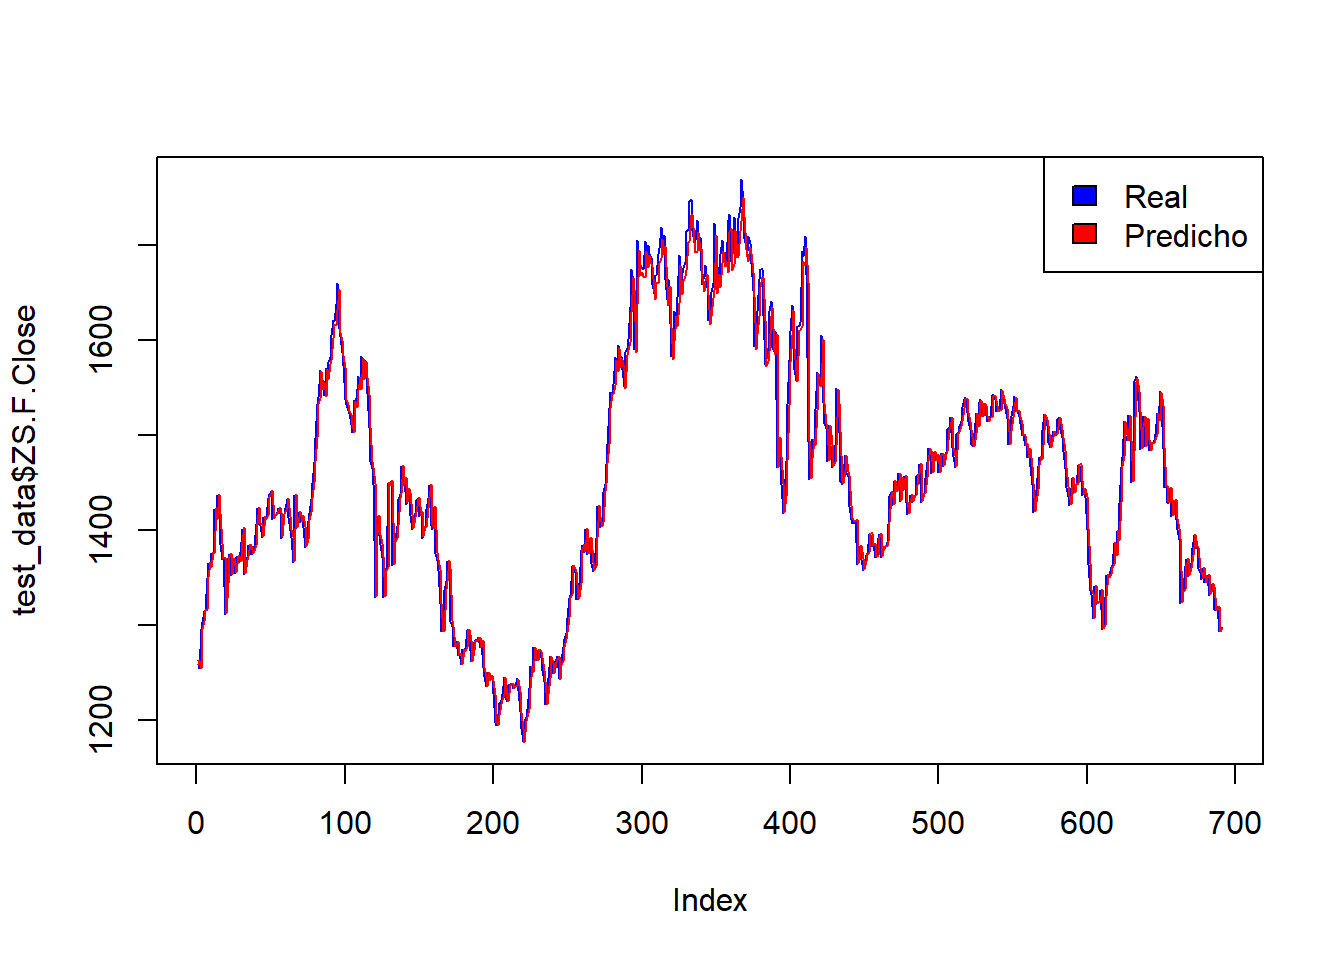
\includegraphics{bookdown-demo_files/figure-latex/unnamed-chunk-36-1.pdf}

Conclusiones:

\begin{itemize}
\item
  Ajuste Exitoso: El modelo se ajusta bien a los datos, reflejando su tendencia y estructura.
\item
  Posible Overfitting: Un ajuste muy cercano puede indicar sobreajuste, lo que afectaría la generalización en datos futuros.
\item
  Evaluación Complementaria: Más allá de gráficos, usar métricas cuantitativas (como MSE o MAE) es esencial para una evaluación objetiva.
\item
  Aplicabilidad a Corto Plazo: El modelo puede ser útil para predicciones a corto plazo, pero podría necesitar reentrenamiento para proyecciones más lejanas.
\end{itemize}

\hypertarget{jordan}{%
\chapter{Jordan}\label{jordan}}

Una red neuronal Jordan es un tipo especial de red neuronal que puede recordar información pasada para ayudar en predicciones futuras. En lugar de simplemente tomar una entrada y producir una salida, esta red toma tanto la entrada actual como su propia salida anterior para hacer su próxima predicción. Es como si tuviera una pequeña memoria de lo que hizo anteriormente.

Imagina que intentas predecir el clima. En lugar de solo mirar el clima de hoy, también consideras lo que predijiste ayer. Esa es la idea detrás de la red Jordan

\begin{Shaded}
\begin{Highlighting}[]
\CommentTok{\# Cargar los paquetes necesarios}
\CommentTok{\# install.packages("neuralnet")}
\CommentTok{\# install.packages("xts")}
\FunctionTok{library}\NormalTok{(neuralnet)}
\FunctionTok{library}\NormalTok{(xts)}

\CommentTok{\# Acceder a la columna de cierre}
\NormalTok{data }\OtherTok{\textless{}{-}} \FunctionTok{data.frame}\NormalTok{(}\AttributeTok{ZS.F.Close =} \FunctionTok{as.vector}\NormalTok{(soybean\_xts[, }\StringTok{"ZS.F.Close"}\NormalTok{]))}

\CommentTok{\# Crear un retraso (lag) para las series temporales y también un retraso para la variable objetivo}
\NormalTok{data}\SpecialCharTok{$}\NormalTok{lag\_close }\OtherTok{\textless{}{-}} \FunctionTok{c}\NormalTok{(}\ConstantTok{NA}\NormalTok{, }\FunctionTok{head}\NormalTok{(data}\SpecialCharTok{$}\NormalTok{ZS.F.Close, }\SpecialCharTok{{-}}\DecValTok{1}\NormalTok{))}
\NormalTok{data}\SpecialCharTok{$}\NormalTok{lag\_output }\OtherTok{\textless{}{-}} \FunctionTok{c}\NormalTok{(}\ConstantTok{NA}\NormalTok{, }\ConstantTok{NA}\NormalTok{, }\FunctionTok{head}\NormalTok{(data}\SpecialCharTok{$}\NormalTok{ZS.F.Close, }\SpecialCharTok{{-}}\DecValTok{2}\NormalTok{))  }\CommentTok{\# Esto simula la idea de la red Jordan}

\CommentTok{\# Eliminar las primeras filas, ya que tendrán NA por el retraso}
\NormalTok{data }\OtherTok{\textless{}{-}}\NormalTok{ data[}\SpecialCharTok{{-}}\FunctionTok{c}\NormalTok{(}\DecValTok{1}\NormalTok{,}\DecValTok{2}\NormalTok{),]}

\CommentTok{\# Dividir los datos en conjuntos de entrenamiento y prueba}
\NormalTok{train\_indices }\OtherTok{\textless{}{-}} \DecValTok{1}\SpecialCharTok{:}\NormalTok{(}\FunctionTok{nrow}\NormalTok{(data) }\SpecialCharTok{*} \FloatTok{0.8}\NormalTok{)}
\NormalTok{train\_data }\OtherTok{\textless{}{-}}\NormalTok{ data[train\_indices,]}
\NormalTok{test\_data }\OtherTok{\textless{}{-}}\NormalTok{ data[}\SpecialCharTok{{-}}\NormalTok{train\_indices,]}

\CommentTok{\# Normalizar los datos}
\NormalTok{maxs }\OtherTok{\textless{}{-}} \FunctionTok{apply}\NormalTok{(train\_data, }\DecValTok{2}\NormalTok{, max)}
\NormalTok{mins }\OtherTok{\textless{}{-}} \FunctionTok{apply}\NormalTok{(train\_data, }\DecValTok{2}\NormalTok{, min)}
\NormalTok{train\_data\_norm }\OtherTok{\textless{}{-}} \FunctionTok{as.data.frame}\NormalTok{(}\FunctionTok{scale}\NormalTok{(train\_data, }\AttributeTok{center=}\NormalTok{mins, }\AttributeTok{scale=}\NormalTok{maxs}\SpecialCharTok{{-}}\NormalTok{mins))}
\NormalTok{test\_data\_norm }\OtherTok{\textless{}{-}} \FunctionTok{as.data.frame}\NormalTok{(}\FunctionTok{scale}\NormalTok{(test\_data, }\AttributeTok{center=}\NormalTok{mins, }\AttributeTok{scale=}\NormalTok{maxs}\SpecialCharTok{{-}}\NormalTok{mins))}

\CommentTok{\# Entrenar una red "Jordan{-}inspired" }
\FunctionTok{set.seed}\NormalTok{(}\DecValTok{123}\NormalTok{)}
\NormalTok{nn }\OtherTok{\textless{}{-}} \FunctionTok{neuralnet}\NormalTok{(ZS.F.Close }\SpecialCharTok{\textasciitilde{}}\NormalTok{ lag\_close }\SpecialCharTok{+}\NormalTok{ lag\_output, }\AttributeTok{data=}\NormalTok{train\_data\_norm, }\AttributeTok{hidden=}\DecValTok{5}\NormalTok{, }\AttributeTok{algorithm=}\StringTok{"rprop+"}\NormalTok{, }\AttributeTok{linear.output=}\ConstantTok{TRUE}\NormalTok{, }\AttributeTok{likelihood=}\ConstantTok{TRUE}\NormalTok{)}

\CommentTok{\# Hacer predicciones}
\NormalTok{test\_data\_for\_pred }\OtherTok{\textless{}{-}} \FunctionTok{data.frame}\NormalTok{(}\AttributeTok{lag\_close =}\NormalTok{ test\_data\_norm}\SpecialCharTok{$}\NormalTok{lag\_close, }\AttributeTok{lag\_output =}\NormalTok{ test\_data\_norm}\SpecialCharTok{$}\NormalTok{lag\_output)}
\NormalTok{predicted\_norm }\OtherTok{\textless{}{-}} \FunctionTok{compute}\NormalTok{(nn, test\_data\_for\_pred)}

\CommentTok{\# Des{-}normalizar las predicciones}
\NormalTok{predicted }\OtherTok{\textless{}{-}}\NormalTok{ (predicted\_norm}\SpecialCharTok{$}\NormalTok{net.result }\SpecialCharTok{*}\NormalTok{ (maxs[}\DecValTok{1}\NormalTok{] }\SpecialCharTok{{-}}\NormalTok{ mins[}\DecValTok{1}\NormalTok{])) }\SpecialCharTok{+}\NormalTok{ mins[}\DecValTok{1}\NormalTok{]}

\CommentTok{\# Comparar las predicciones con los datos reales}
\FunctionTok{plot}\NormalTok{(test\_data}\SpecialCharTok{$}\NormalTok{ZS.F.Close, }\AttributeTok{type=}\StringTok{"l"}\NormalTok{, }\AttributeTok{col=}\StringTok{"blue"}\NormalTok{)}
\FunctionTok{lines}\NormalTok{(predicted, }\AttributeTok{col=}\StringTok{"red"}\NormalTok{)}
\FunctionTok{legend}\NormalTok{(}\StringTok{"topright"}\NormalTok{, }\AttributeTok{legend=}\FunctionTok{c}\NormalTok{(}\StringTok{"Real"}\NormalTok{, }\StringTok{"Predicho"}\NormalTok{), }\AttributeTok{fill=}\FunctionTok{c}\NormalTok{(}\StringTok{"blue"}\NormalTok{, }\StringTok{"red"}\NormalTok{))}
\end{Highlighting}
\end{Shaded}

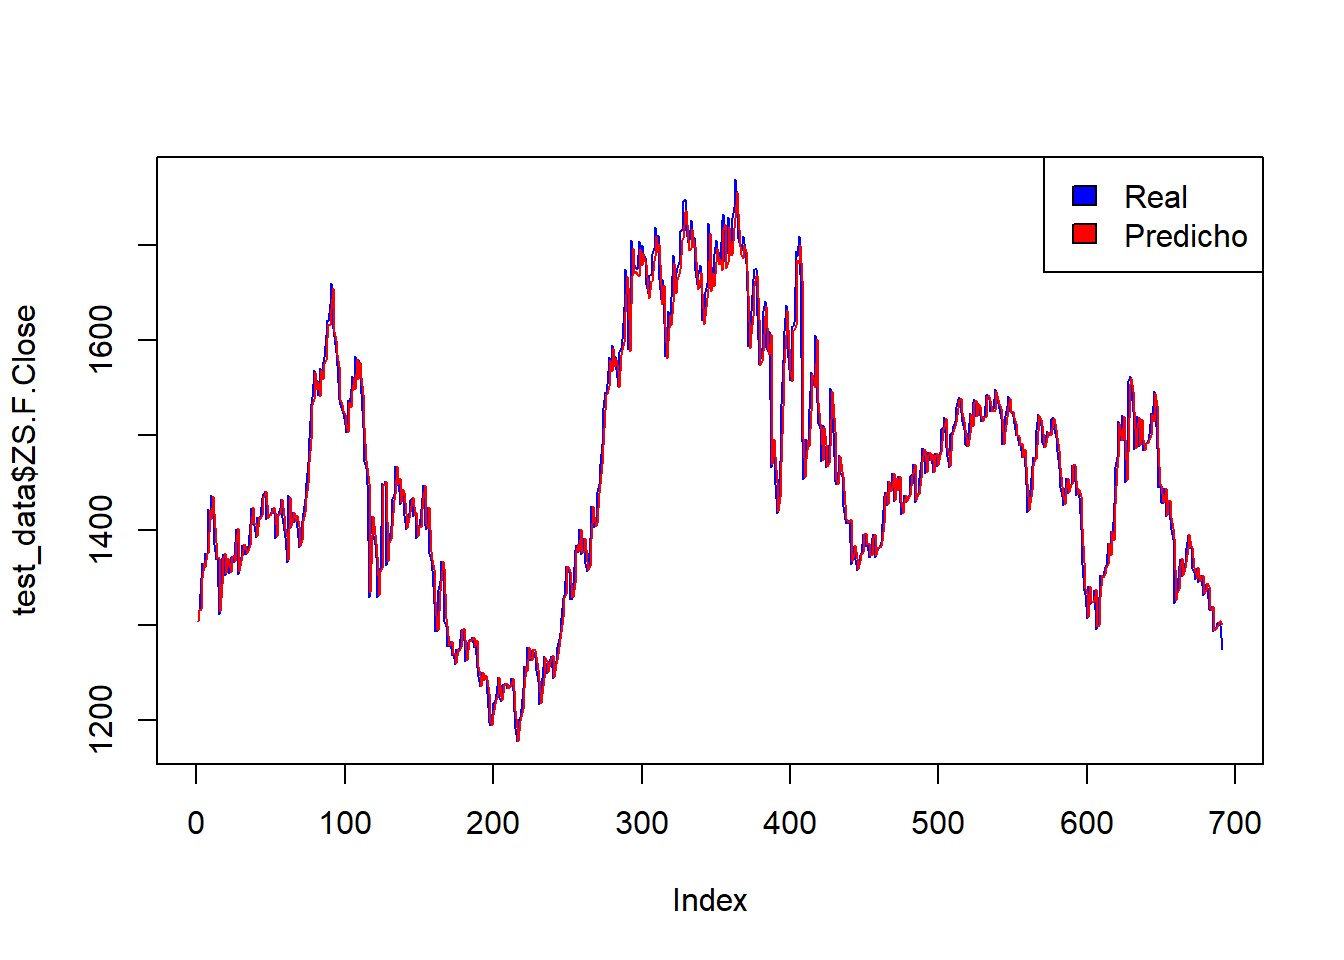
\includegraphics{bookdown-demo_files/figure-latex/unnamed-chunk-37-1.pdf}

Conclusiones:

El modelo predice con exactitud,funciona bien en datos no vistos,es equilibrado, no solo memoriza los datos de entrenamiento,los datos usados son pertinentes para la tarea, puede ser aplicado en situaciones reales, a pesar de los buenos resultados, siempre es esencial hacer análisis.

\hypertarget{final-words}{%
\chapter{Final Words}\label{final-words}}

We have finished a nice book.

  \bibliography{book.bib,packages.bib}

\end{document}
